\documentclass[12pt,reqno,oneside,hidelinks]{article}
% \documentclass[12pt, final]{siamonline171218}
% \usepackage[pdfborder={0 0 0.5 [3 2]}]{hyperref}%
\usepackage[left=0.85in,right=0.85in,top=0.75in,bottom=1in]{geometry}%
\usepackage{amsmath}
\usepackage{amssymb}
\usepackage{amsthm}
\usepackage{graphicx}
\usepackage{enumerate}
\usepackage{float}
\usepackage{bm}
\usepackage[stable]{footmisc}

\usepackage{packages}
\usepackage{wrapfig}
\usepackage{subfigure}
\usepackage[font=footnotesize]{caption}

% \newtheorem{theorem}{Theorem}
% \newtheorem{lemma}[theorem]{Lemma}
% \newtheorem{corollary}{Corollary}

% \theoremstyle{definition}
% \newtheorem{definition}[theorem]{Definition}

% \theoremstyle{remark}
% \newtheorem{remark}[theorem]{Remark}

\def\noi{\noindent}
\def\T{{\mathbb T}}
\def\R{{\mathbb R}}
\def\N{{\mathbb N}}
\def\Z{{\mathbb Z}}
\def\C{{\mathbb C}}
\def\Q{\mathbb{Q}}

\newcommand{\xvec}{\mathbf{x}}
\newcommand{\vK}{\bm{\mathit{K}}}
\newcommand{\calP}{\mathcal{P}}
\newcommand{\calA}{\mathcal{A}}

\setlength{\parindent}{0em}
\setlength{\parskip}{1em}
\renewcommand{\baselinestretch}{1.1}

\title{Research Statement}
\date{\vspace{-12ex}}

\begin{document}

\thispagestyle{empty}

\section*{Research statement}

My main research focus is on understanding patterns and coherent structures arising in the natural sciences and engineering. Mathematically, these are described by nonlinear evolution equations, which take the form of partial differential equations (PDEs) or systems of ordinary differential equations (ODEs). Most of the systems I study are nonlinear wave equations, which describe the time evolution of a function representing a wave profile. Coherent structures are spatial patterns which maintain their shape as the system evolves in time. Examples of coherent structures include solitary waves, which are localized disturbances that propagate at a constant velocity; wavetrains, which are periodic disturbances that also propagate at a constant velocity; and breathers, which are disturbances that are localized in space but oscillate in time. Solitary waves have been a topic of interest since the 19th century, when John Scott Russell observed a single, large surface wave on the Edinburgh-Glasgow Union Canal in Scotland; the wave propagated along the canal undisturbed for a few miles before eventually decaying. This phenomenon was explained mathematically by the Korteweg–De Vries (KdV) equation 
\[
u_t + u_{xxx} + 6 u u_x = 0,
\]
which has both solitary wave and wavetrain solutions.
\begin{figure}[H]
    \centering
    \begin{tabular}{cc}
        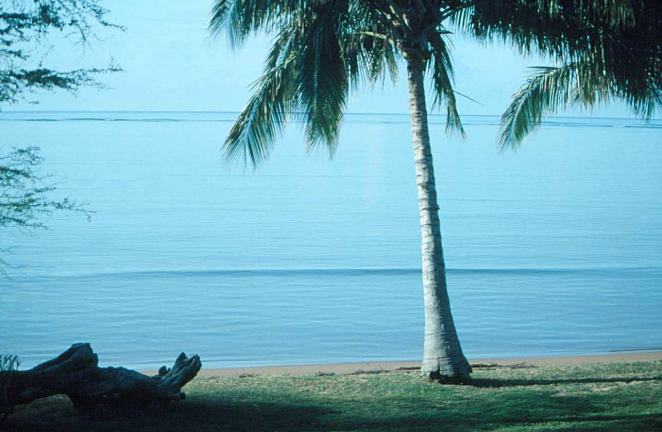
\includegraphics[width=7cm]{images/SolitaryWaveHawaii.png} &
        % 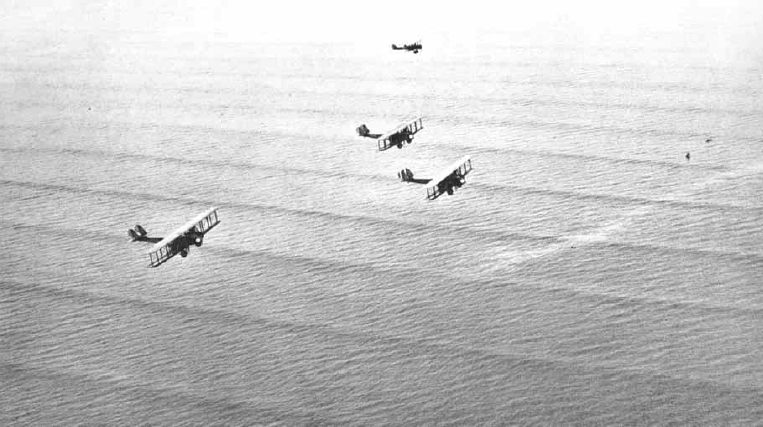
\includegraphics[width=7cm]{images/cnoidalwaves.png} 
        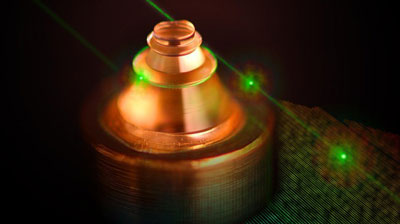
\includegraphics[width=8.1cm]{images/resonator.jpg} 
        % 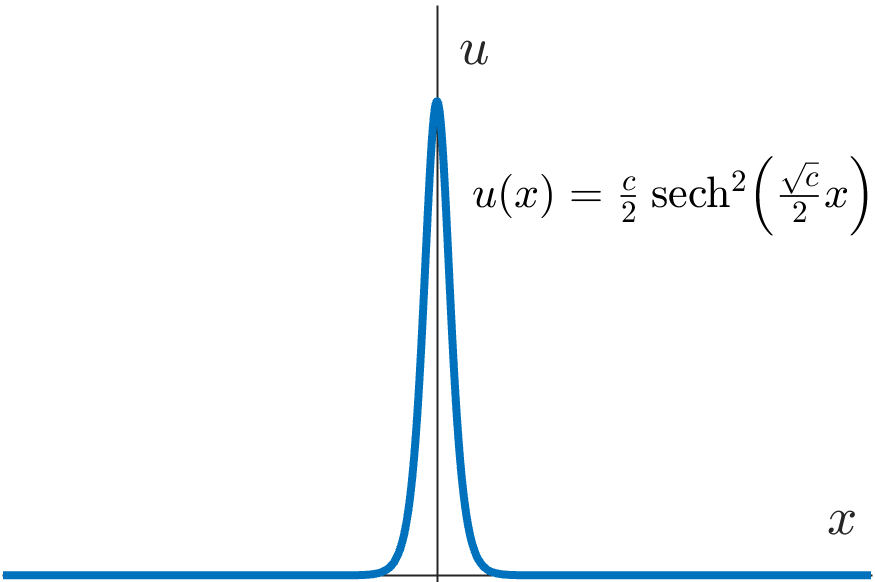
\includegraphics[width=7cm]{images/kdvsoliton.png} &
        % 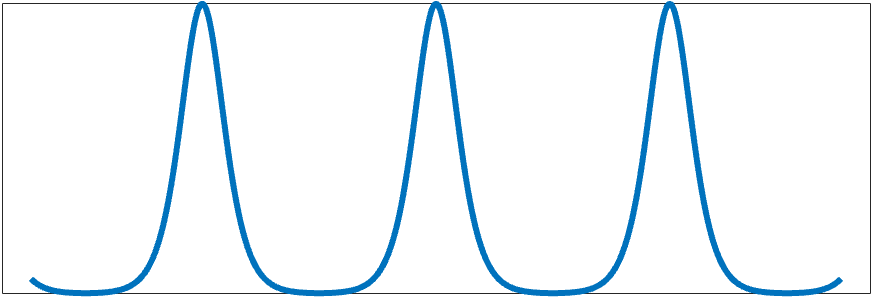
\includegraphics[width=7cm]{images/kdvcn.png}      
    \end{tabular}
    \caption{Solitary wave off the coast of Hawaii \cite{Andriopoulos2009} (left). Optical solitons in a microresonator \cite{MarinPalomo2017} (right) }
    \label{fig:solitarywaves}
\end{figure}
Although solitary waves were originally discovered as a water wave phenomenon, they have applications in many fields, including fiber optics, plasma physics, quantum mechanics, molecular biology, and neuroscience (\cref{fig:solitarywaves}). More generally, many nonlinear, dispersive PDEs exhibit solitary wave solutions. My research falls into two broad categories: multi-pulse solitary waves in Hamiltonian systems, and coherent structures in optical lattices. Beyond those, I have also explored bifurcation structures in a neural network model and systems of coupled oscillators. In addition to summarizing my research, I will also highlight future research directions and ways in which I can involve students in my research program.

\section*{Multi-pulse solitary waves in Hamiltonian systems}

The bulk of my published research concerns coherent structures in Hamiltonian systems; these systems are characterized by a conserved quantity, such as energy, that remains constant in time. At a high level, I start with a simple coherent structure, such as a solitary wave, and use it as a building block to construct more elaborate structures. I then study the stability of these more complicated structures in terms of their underlying geometry, together with properties of the simpler structure. 

The prototypical nonlinear wave equation has a primary solitary wave solution, also known as a primary pulse solution, which looks like a single localized ``bump'' (\cref{fig:kdvpp}, left). In many systems, multi-pulse solutions also exist; these are ``multi-bump'' solitary waves which resemble multiple, well-separated copies of the primary pulse. (Notably, multi-pulse solutions do not exist to the KdV equation). The entire multi-pulse travels as a unit, and maintains its shape unless perturbed. In addition to having applications in nonlinear optics and neuroscience \cite{Evans1982}, multi-pulses are interesting mathematically. In my research, I explore the existence and stability of these multi-pulse structures. A crucial step in this process is determining the spectrum of the linearization of the underlying system about a multi-pulse. When a multi-pulse is perturbed, interactions between the individual pulses in the structure are revealed, which are a consequence of the inherent nonlinearity of the system. The dynamics of these interactions are determined by the eigenvalues of the linearized system and their corresponding eigenfunctions.

\begin{figure}[H]
    \centering
    \begin{tabular}{cc}
        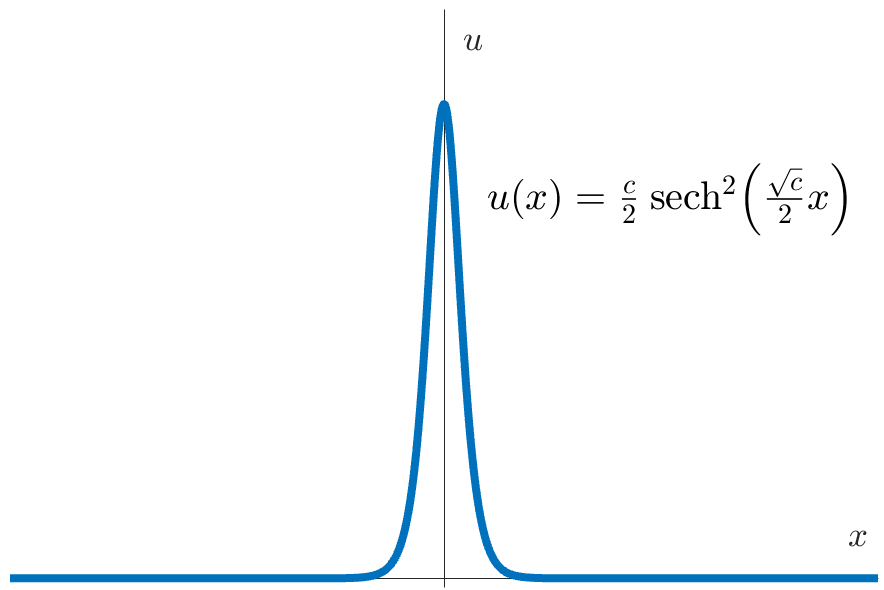
\includegraphics[width=6cm]{images/KdVsolitoneq.png} \hspace{2cm} &
        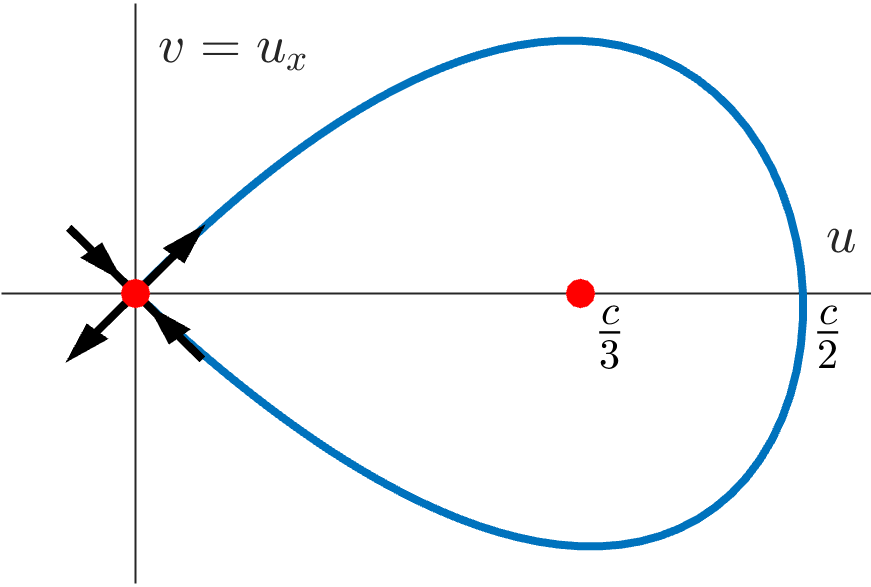
\includegraphics[width=6cm]{images/KdVphaseportait.png} 
    \end{tabular}
    \caption{Primary solitary wave solution $u(x)$ to the KdV equation. Left panel is plot of $u$ vs $x$. Right panel is plot of $u_x$ vs $u$, showing solitary wave as a homoclinic orbit.}
    \label{fig:kdvpp}
\end{figure}

My primary mathematical approach comes from spatial dynamics. From this viewpoint, a solitary wave is a homoclinic orbit evolving in the spatial variable $x$. For example, the solitary wave solution $u(x)$ to the KdV equation which travels to the right with constant speed $c$ (\cref{fig:kdvpp}, left panel) is a solution to the second order ODE $u_{xx} + 3 u^2 - c u = 0$. This can be written as the two-dimensional dynamical system 
\[
\frac{d}{dx}\begin{pmatrix}u\\v\end{pmatrix}
= \begin{pmatrix}v \\ cu - 3u^2\end{pmatrix}
\]
by taking $v = u_x$. From this perspective, the solitary wave solution $(u(x), v(x))$ is a homoclinic orbit connecting the unstable and stable manifolds of the saddle equilibrium point at the origin (\cref{fig:kdvpp}, right panel), which represents the rest state of the system. 

From a spatial dynamics perspective, multi-pulses are multi-loop homoclinic orbits. Multi-pulses can be constructed using Lin's method \cite{Lin2008}, a version of the Lyapunov-Schmidt method which can be used to find solutions that are close to a homoclinic orbit. Heuristically, this process involves ``gluing together'' multiple copies of the primary pulse solution end-to-end using small remainder functions (\cref{fig:linsmethod}). Lin's method can also be used to construct periodic orbits and multi-loop periodic orbits. The existence of multi-pulse solutions is constrained by the geometry of the primary pulse and the underlying system. In \cref{fig:linsmethod}, for example, multi-pulses can only exist when the tail oscillations of the individual pulses overlap in phase.
\begin{figure}
    \centering
    \begin{tabular}{cc}
        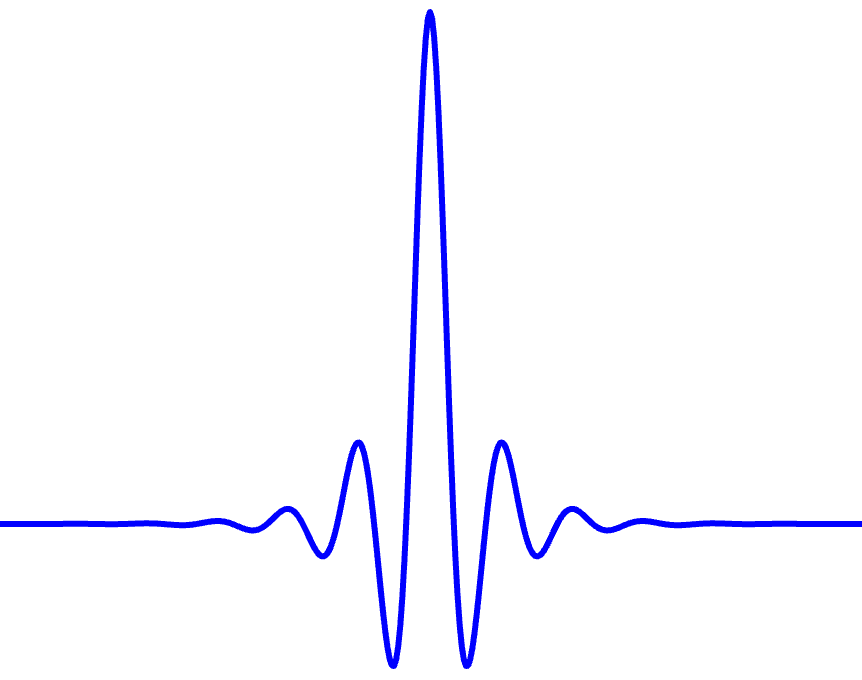
\includegraphics[width=5.65cm]{images/linchen1.png} &
        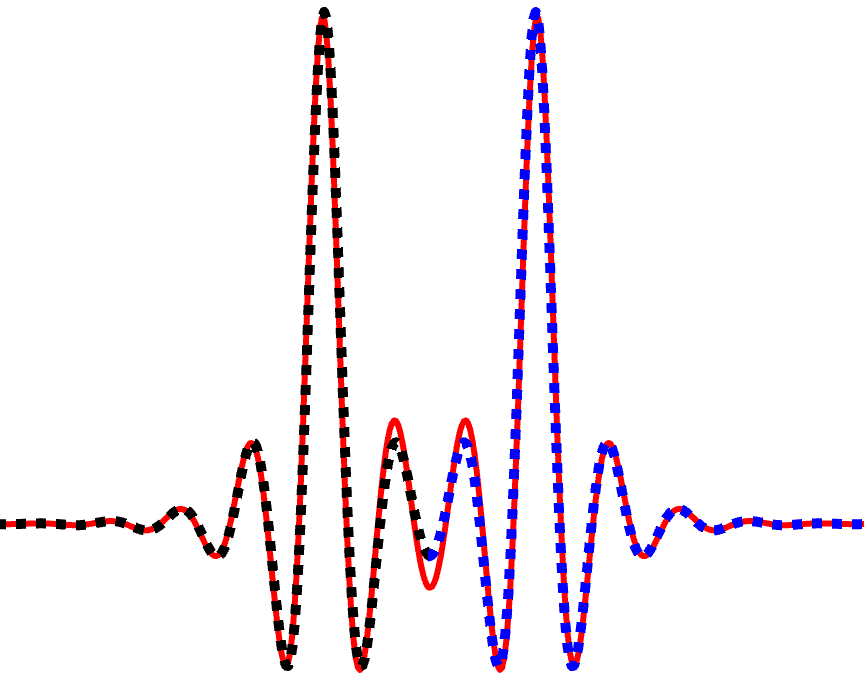
\includegraphics[width=5.65cm]{images/linchen2.png} 
    \end{tabular}
    \caption{Cartoon illustrating construction of a double pulse solution using Lin's method. Left panel shows primary pulse solution. Right panel shows two copies of the primary pulse solution (black and blue dotted lines) placed end-to-end. Double pulse solution (red solid line) is close, but not equal, to this.}
    \label{fig:linsmethod}
\end{figure}

\begin{wrapfigure}[7]{R}{6cm}
    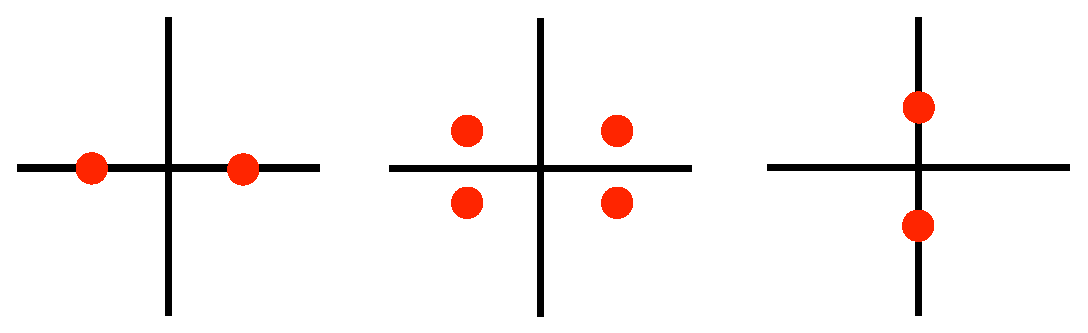
\includegraphics[width=6cm]{images/inteigpattern.eps}
    \caption{Possible interaction eigenvalue patterns in a Hamiltonian system.} 
    \label{fig:inteigpattern}
\end{wrapfigure}
The first step in the stability analysis of a multi-pulse solution is computing the spectrum of the linearization of the underlying system about the solution. In general, each pulse that is added to a multi-pulse structure is associated with one or more eigenvalues in the spectrum \cite{Sandstede1998}, which I call interaction eigenvalues, since they result from nonlinear interactions between the tails of neighboring pulses. The systems I study are Hamiltonian, which are not covered by the results of \cite{Sandstede1998}. On one hand, the Hamiltonian structure is very helpful, since all eigenvalues must come in quartets of the form $\pm \alpha \pm \beta i$. This means that each additional set of interaction eigenvalues must occur in one of the three patterns in \cref{fig:inteigpattern}. On the other hand, the presence of any eigenvalue with nonzero real part implies that there is an unstable eigenvalue with positive real part. This means that Hamiltonian systems cannot be dissipative, which makes stability analysis more difficult. My main results relate the spectral pattern of the interaction eigenvalues to the underlying geometry of the multi-pulse. In all cases, the spectral pattern is determined by this geometry. 

\begin{figure}[H]
    \centering
    \begin{tabular}{ccc}
        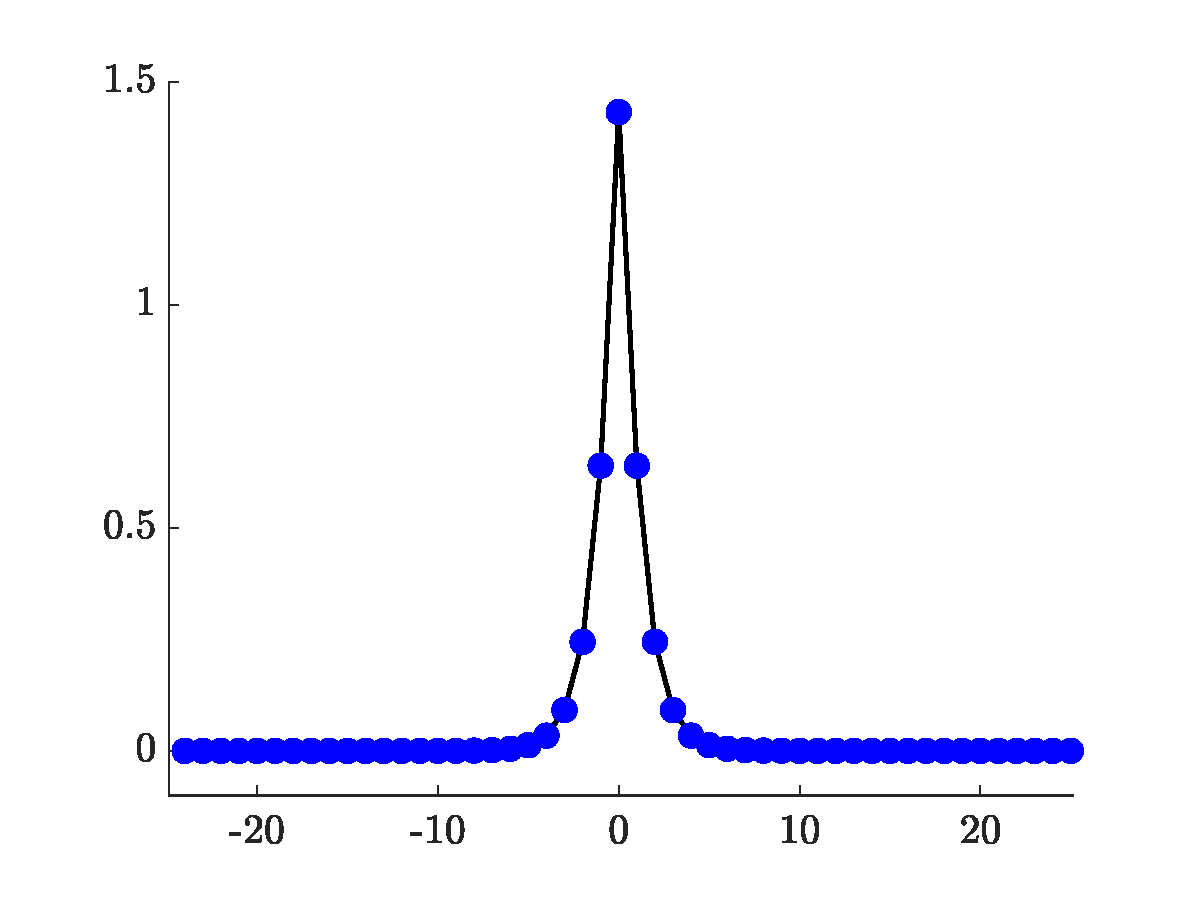
\includegraphics[width=5cm]{images/DNLSprimary.eps} &
        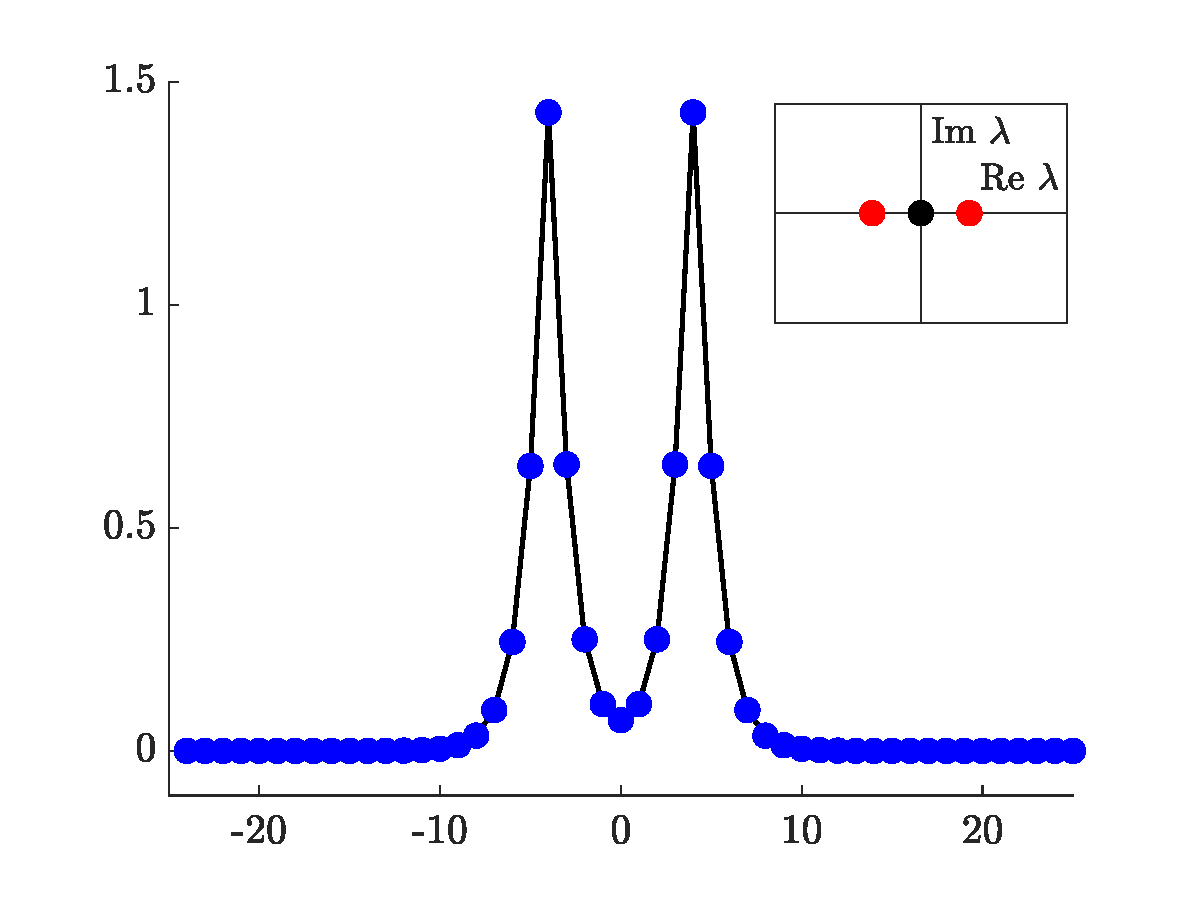
\includegraphics[width=5cm]{images/DNLSunstable2p.eps} &
        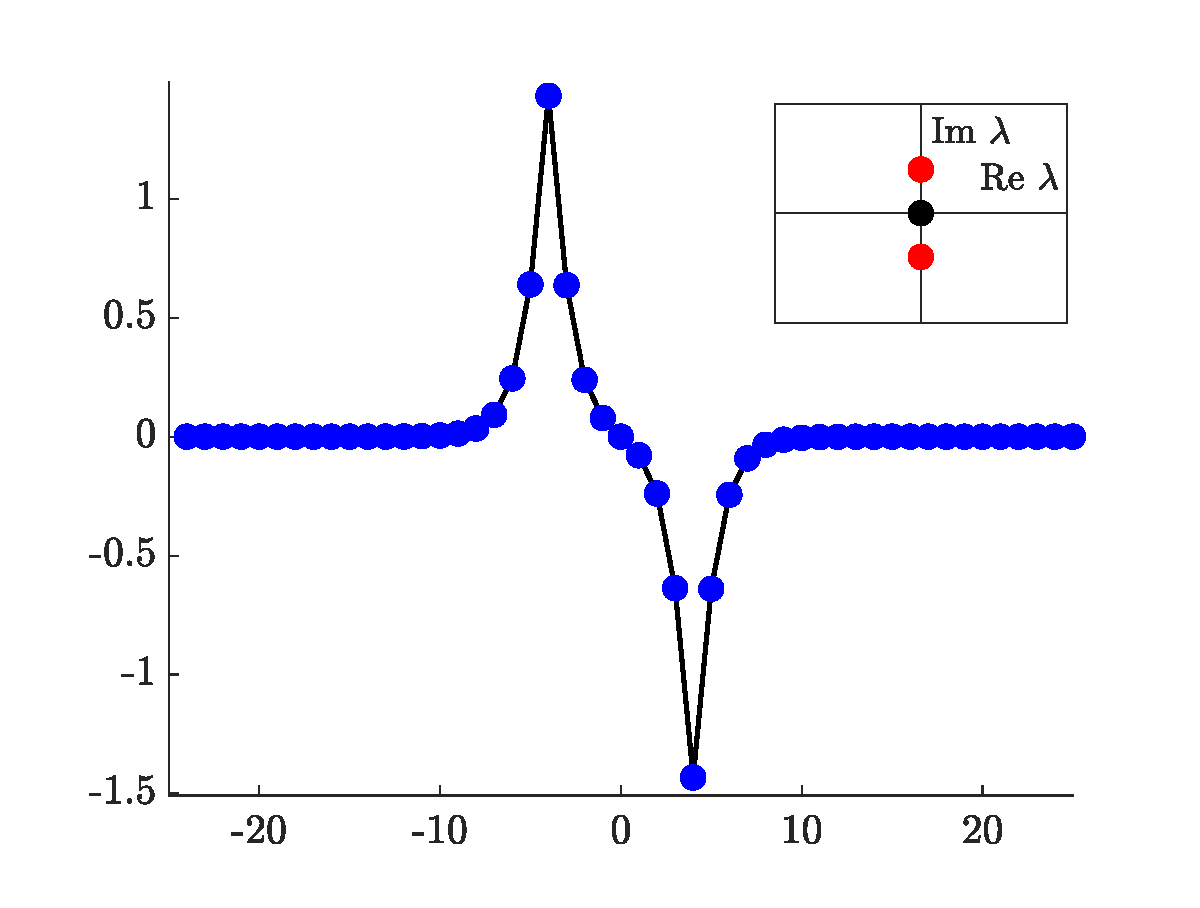
\includegraphics[width=5cm]{images/DNLSstable2p.eps} 
    \end{tabular}
    \caption{Primary pulse (left), out-of-phase double pulse (middle), and in-phase double pulse (right) solutions for DNLS. Interaction eigenvalue patterns for double pulses are shown in insets. Black dot is a kernel eigenvalue with algebraic multiplicity 2.}
    \label{fig:DNLS2p}
\end{figure}

My work makes extensive use of numerical analysis, both to generate hypotheses and to verify analytical results. For multi-pulses, I start by computing the primary solitary wave solution, which either involves numerical parameter continuation from a known solution or an energy minimization method \cite{Chamard2011}. I then splice together multiple copies of the primary solitary wave and use a root-finding method such as conjugate gradient to construct the multi-pulse solution. For stability analysis, I compute the spectrum using an eigenvalue solver on an appropriate discretization of the linearized system. I will highlight four systems I have studied: the discrete nonlinear Schr\"odinger equation, the Chen-McKenna suspension bridge equation, the fifth-order KdV equation, and a fourth order nonlinear Schr\"odinger equation. I will then mention some more recent work, and suggest some future avenues of research.

\subsection*{Discrete nonlinear Schr\"odinger equation}

The discrete nonlinear Schr{\"o}dinger equation (DNLS) 
\begin{align*}
    i \frac{d}{dt} u_n + d(u_{n+1} - 2 u_n + u_{n-1}) + |u_n|^2 u_n && n \in \mathbb{Z}
\end{align*}
is the discrete analogue to the nonlinear Schr{\"o}dinger equation (NLS) on the integer lattice. In addition to being a fundamental model of a nonlinear dynamical system on a lattice, DNLS has applications to nonlinear optics and condensed matter physics \cite{Kevrekidis2009}. The parameter $d$ quantifies the degree of coupling between adjacent lattice sites.  For all values of $d$, DNLS has a stable, primary pulse solution (\cref{fig:DNLS2p}, left panel). Provided that the individual peaks are separated by a sufficiently large number of lattice points, I use Lin's method to prove that multi-pulse solutions exist as long as the following geometric constraint is satisfied: neighboring peaks must either be out-of-phase or in-phase \cite[Theorem 4]{Parker2020}. Furthermore, I prove this that geometry determines the stability of multi-pulses \cite[Theorem 5]{Parker2020}. For double pulses, the in-phase double pulse is unstable, since there is eigenvalue with positive real part, and the out-of-phase double pulse is neutrally stable, since the entire spectrum lies on the imaginary axis (\cref{fig:DNLS2p}). For general multi-pulses, the entire structure is unstable if any pair of neighboring peaks is in-phase. The only neutrally stable multi-pulses are those in which every pair of neighboring peaks is out-of-phase. The proof of this result uses Lin's method to construct the eigenfunctions corresponding to the interaction eigenvalues. This reduces the spectral problem to finding the eigenvalues of a matrix.

\begin{figure}
    \centering
    \begin{tabular}{cc}
        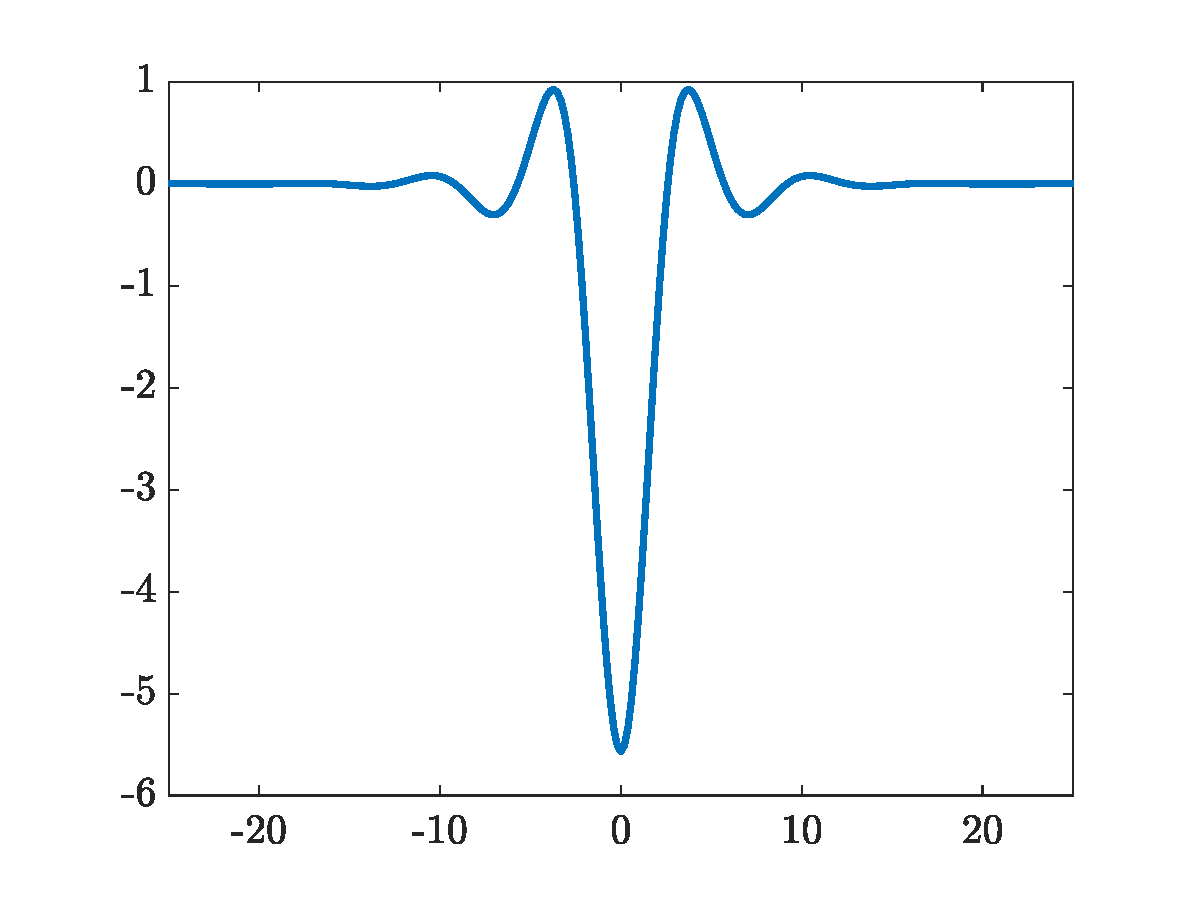
\includegraphics[width=7cm]{images/chen1p.eps} &
        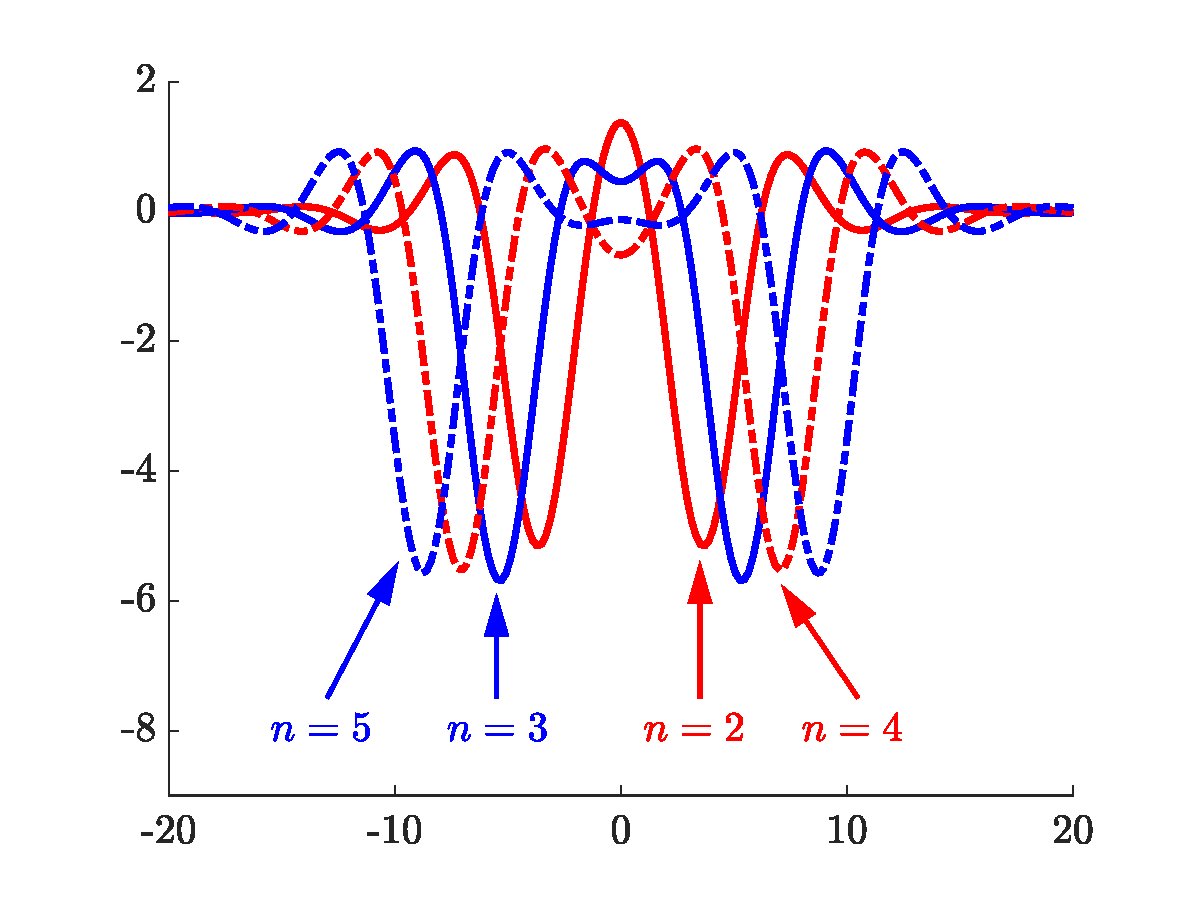
\includegraphics[width=7cm]{images/chenDPall.eps} \\
        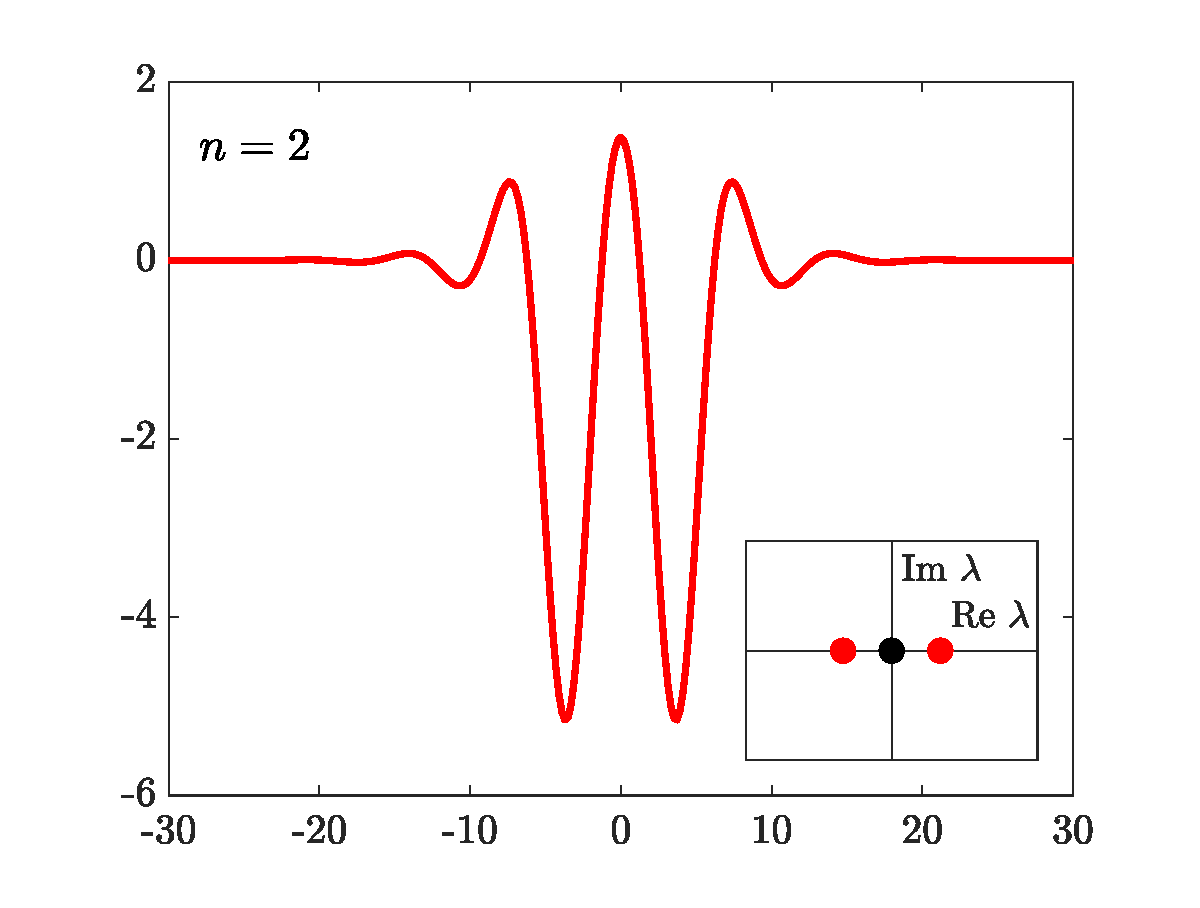
\includegraphics[width=7cm]{images/chen2punstable.eps} &
        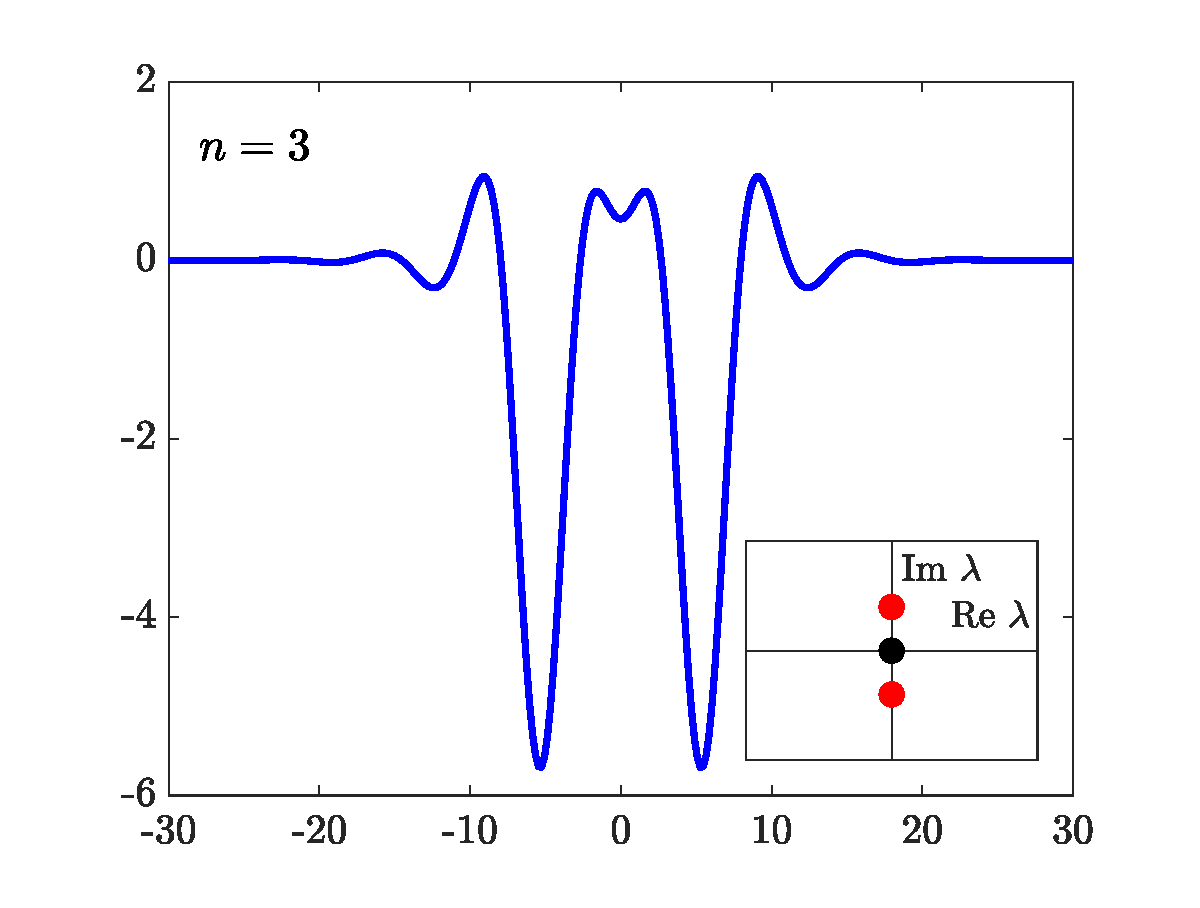
\includegraphics[width=7cm]{images/chen2pstable.eps} 
    \end{tabular}
    \caption{Primary pulse solution for Chen-Mckenna (top left). First four double pulse solutions (top right). Unstable double pulse for $n=2$ (bottom left) and neutrally stable double pulse for $n=3$ (bottom right). Interaction eigenvalue patterns for double pulses are shown in insets. Black dot is a kernel eigenvalue with algebraic multiplicity 2.}
    \label{fig:chen2p}
\end{figure}

\subsection*{Chen-McKenna suspension bridge equation}

The Chen-McKenna suspension bridge equation 
\begin{align*}
    u_{tt} + u_{xxxx} + \mathrm{e}^{u-1} - 1 &= 0 
\end{align*}
is a smooth approximation to a model for waves propagating on an infinitely long suspended beam, and is motivated by observations of traveling waves on suspension bridges \cite{McKenna1990,Chen1997}. For wave speeds $c$ between 0 and $\sqrt{2}$, a primary solitary wave solution exists \cite{Berg2018}, which has exponentially decaying, oscillatory tails (\cref{fig:chen2p}, top left). Provided that the individual peaks are sufficiently well separated, multi-pulse solutions exist as long as the following geometric constraint is satisfied: the tail oscillations of neighboring peaks must overlap in-phase (see \cref{fig:chen2p}, top left, and cartoon in \cref{fig:linsmethod}). This constraint is a consequence of a specific alignment of the unstable and stable manifolds which is required for a multi-loop homoclinic orbit to exist. As a result, the distance between consecutive peaks is, to leading order, an integer multiple of a phase parameter. This is illustrated in the top right panel of \cref{fig:chen2p}, which plots the first four double pulse solutions on the same graph. As with DNLS, the stability of multi-pulses depends on their geometry. Double pulses, for example, alternate between unstable (\cref{fig:chen2p}, bottom left, corresponding to even integers) and neutrally stable (\cref{fig:chen2p}, bottom right, corresponding to odd integers). I prove these results using an extension of the Krein matrix \cite{Kapitula2020}, a tool which projects the infinite-dimensional spectral problem onto a finite-dimensional space. 

\subsection*{Fifth order KdV equation}

The fifth-order Korteweg de-Vries equation (KdV5)
\begin{align*}
    u_t - u_{xxxxx} + u_{xxx} + 2 u u_x &= 0
\end{align*} 
is a weakly nonlinear long wave approximation to the capillary-gravity wave problem, and also has applications to plasma physics and laser optics \cite{Pelinovsky2007}. Multi-pulse solutions to KdV5 exist \cite{SandstedeStrut}, but their stability analysis is complicated due to the fact that the essential spectrum for all localized solutions comprises the entire imaginary axis. In particular, this means that any purely imaginary interaction eigenvalues would be embedded in the essential spectrum, which makes them difficult to locate.

To avoid this issue, I impose periodic boundary conditions on the problem and look instead at periodic multi-pulses, which are multi-pulses on a periodic domain. From a spatial dynamics perspective, a periodic multi-pulse is a multi-loop periodic orbit which is close to the primary homoclinic orbit. These are constructed by ``gluing together'' multiple copies of the primary pulse end-to-end in a loop. A periodic double pulse, for example, is constructed by connecting two single pulses together at both ends (\cref{fig:periodic}, left). Since this construction involves two length parameters $X_0$ and $X_1$, there is an extra degree of freedom when compared to double pulses on the real line, which only involve a single length parameter. As a consequence, I prove that periodic double pulses exist in a continuous family, in which asymmetric periodic double pulses (those with $X_0 \neq X_1$) bifurcate from symmetric periodic double pulses (those with $X_0 = X_1$) in a series of pitchfork bifurcations (\cref{fig:periodic}, center) \cite{ParkerKdV}. The advantage of looking at periodic solutions is that the essential spectrum becomes a discrete set of eigenvalues on the imaginary axis (blue open circles in \cref{fig:periodic}, right). Purely imaginary interaction eigenvalues can then lie between these essential spectrum eigenvalues, which avoids the problem of embedded eigenvalues. 

\begin{figure}
    \begin{center}
    \includegraphics[width=7cm]{images/2pulse3d.png} \hspace{-1cm}
    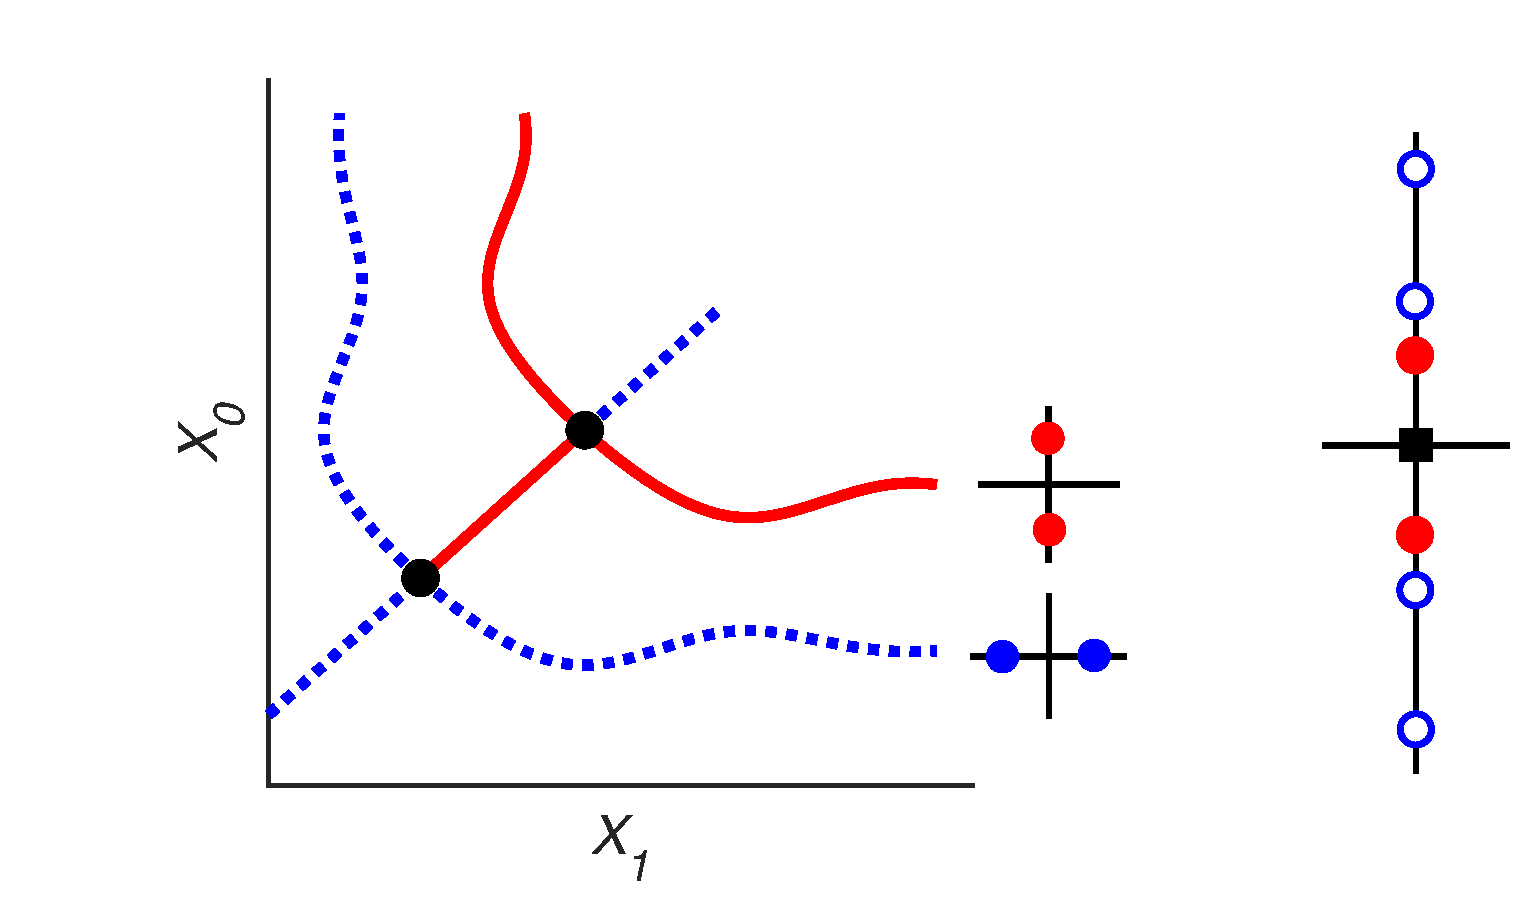
\includegraphics[width=9cm]{images/2pitchforkcoloreig2.eps}
    \end{center}
    \caption{Construction (left) and bifurcation diagram with corresponding interaction eigenvalue pattern (center) of periodic double pulse solutions to KdV5. Spectrum of neutrally stable periodic double pulses (right) comprising interaction eigenvalues (red filled circles), essential spectrum eigenvalues (blue open circles), and kernel eigenvalue with algebraic multiplicity 2 (black square).}
    \label{fig:periodic}
\end{figure}
    
Using Lin's method, I prove that the eigenvalues associated with a periodic multi-pulse can be found by solving a block matrix equation \cite[Theorem 5.3]{ParkerKdV} for $\lambda$. To leading order, this is given by
    \begin{equation}\label{blockmatrix}
    \det \begin{pmatrix}
    K(\lambda) - \frac{1}{2} \lambda \tilde{M} K^+(\lambda) & \lambda^2 M_c I \\
    -\frac{1}{2} \lambda M_c K^+(\lambda) & A - \lambda^2 MI  
    \end{pmatrix} = 0.
    \end{equation}
The essential spectrum eigenvalues are encoded by the matrix $K(\lambda)$, which, to leading order, only depends on the background state and size of the periodic domain; in particular, it is independent of the periodic multi-pulse solution. The interaction eigenvalues are encoded by the matrix $A$, which depends on the geometry of the periodic multi-pulse. $M$, $M_c$, and $\tilde{M}$ are Melnikov-type integrals associated with the primary pulse solution. As long as the periodic domain size is not too large, the interaction eigenvalues and essential spectrum eigenvalues do not interfere with each other. For a periodic double pulse, there is a pair of interaction eigenvalues which is either real or purely imaginary, depending on the geometry of the solution (\cref{fig:periodic}, center). The eigenvalue pattern switches between real and imaginary at the pitchfork bifurcation points.  
    
There is, however, an additional complication in the periodic case. As the periodic domain size $X = X_0 + X_1$ is increased, the essential spectrum eigenvalues move towards the origin. At a critical value of $X$,  there will be a collision between one of the essential spectrum eigenvalues and a purely imaginary interaction eigenvalue. As $X$ is further increased, I prove that a brief instability bubble is formed, wherein the two eigenvalues collide, move off the imaginary axis, trace an approximate circle in the complex plane, and recombine on the imaginary axis in a ``reverse'' collision (see left panel of \cref{fig:kreinbubble1} for a cartoon) \cite[Theorem 5.10]{ParkerKdV}. This instability bubble, which I call a Krein bubble since the eigenvalues involved in the collision have opposite Krein signatures, is a direct consequence of the block matrix reduction. A numerical simulation of the Krein bubble, computed using parameter continuation with the specialized software package AUTO \cite{AUTO}, is shown in the right panel of \cref{fig:kreinbubble1}. The location and size of the Krein bubble in the simulation agree with that predicted by the theory \cite{ParkerKdV}.
    
\begin{figure}
\begin{center}
\begin{tabular}{cc}
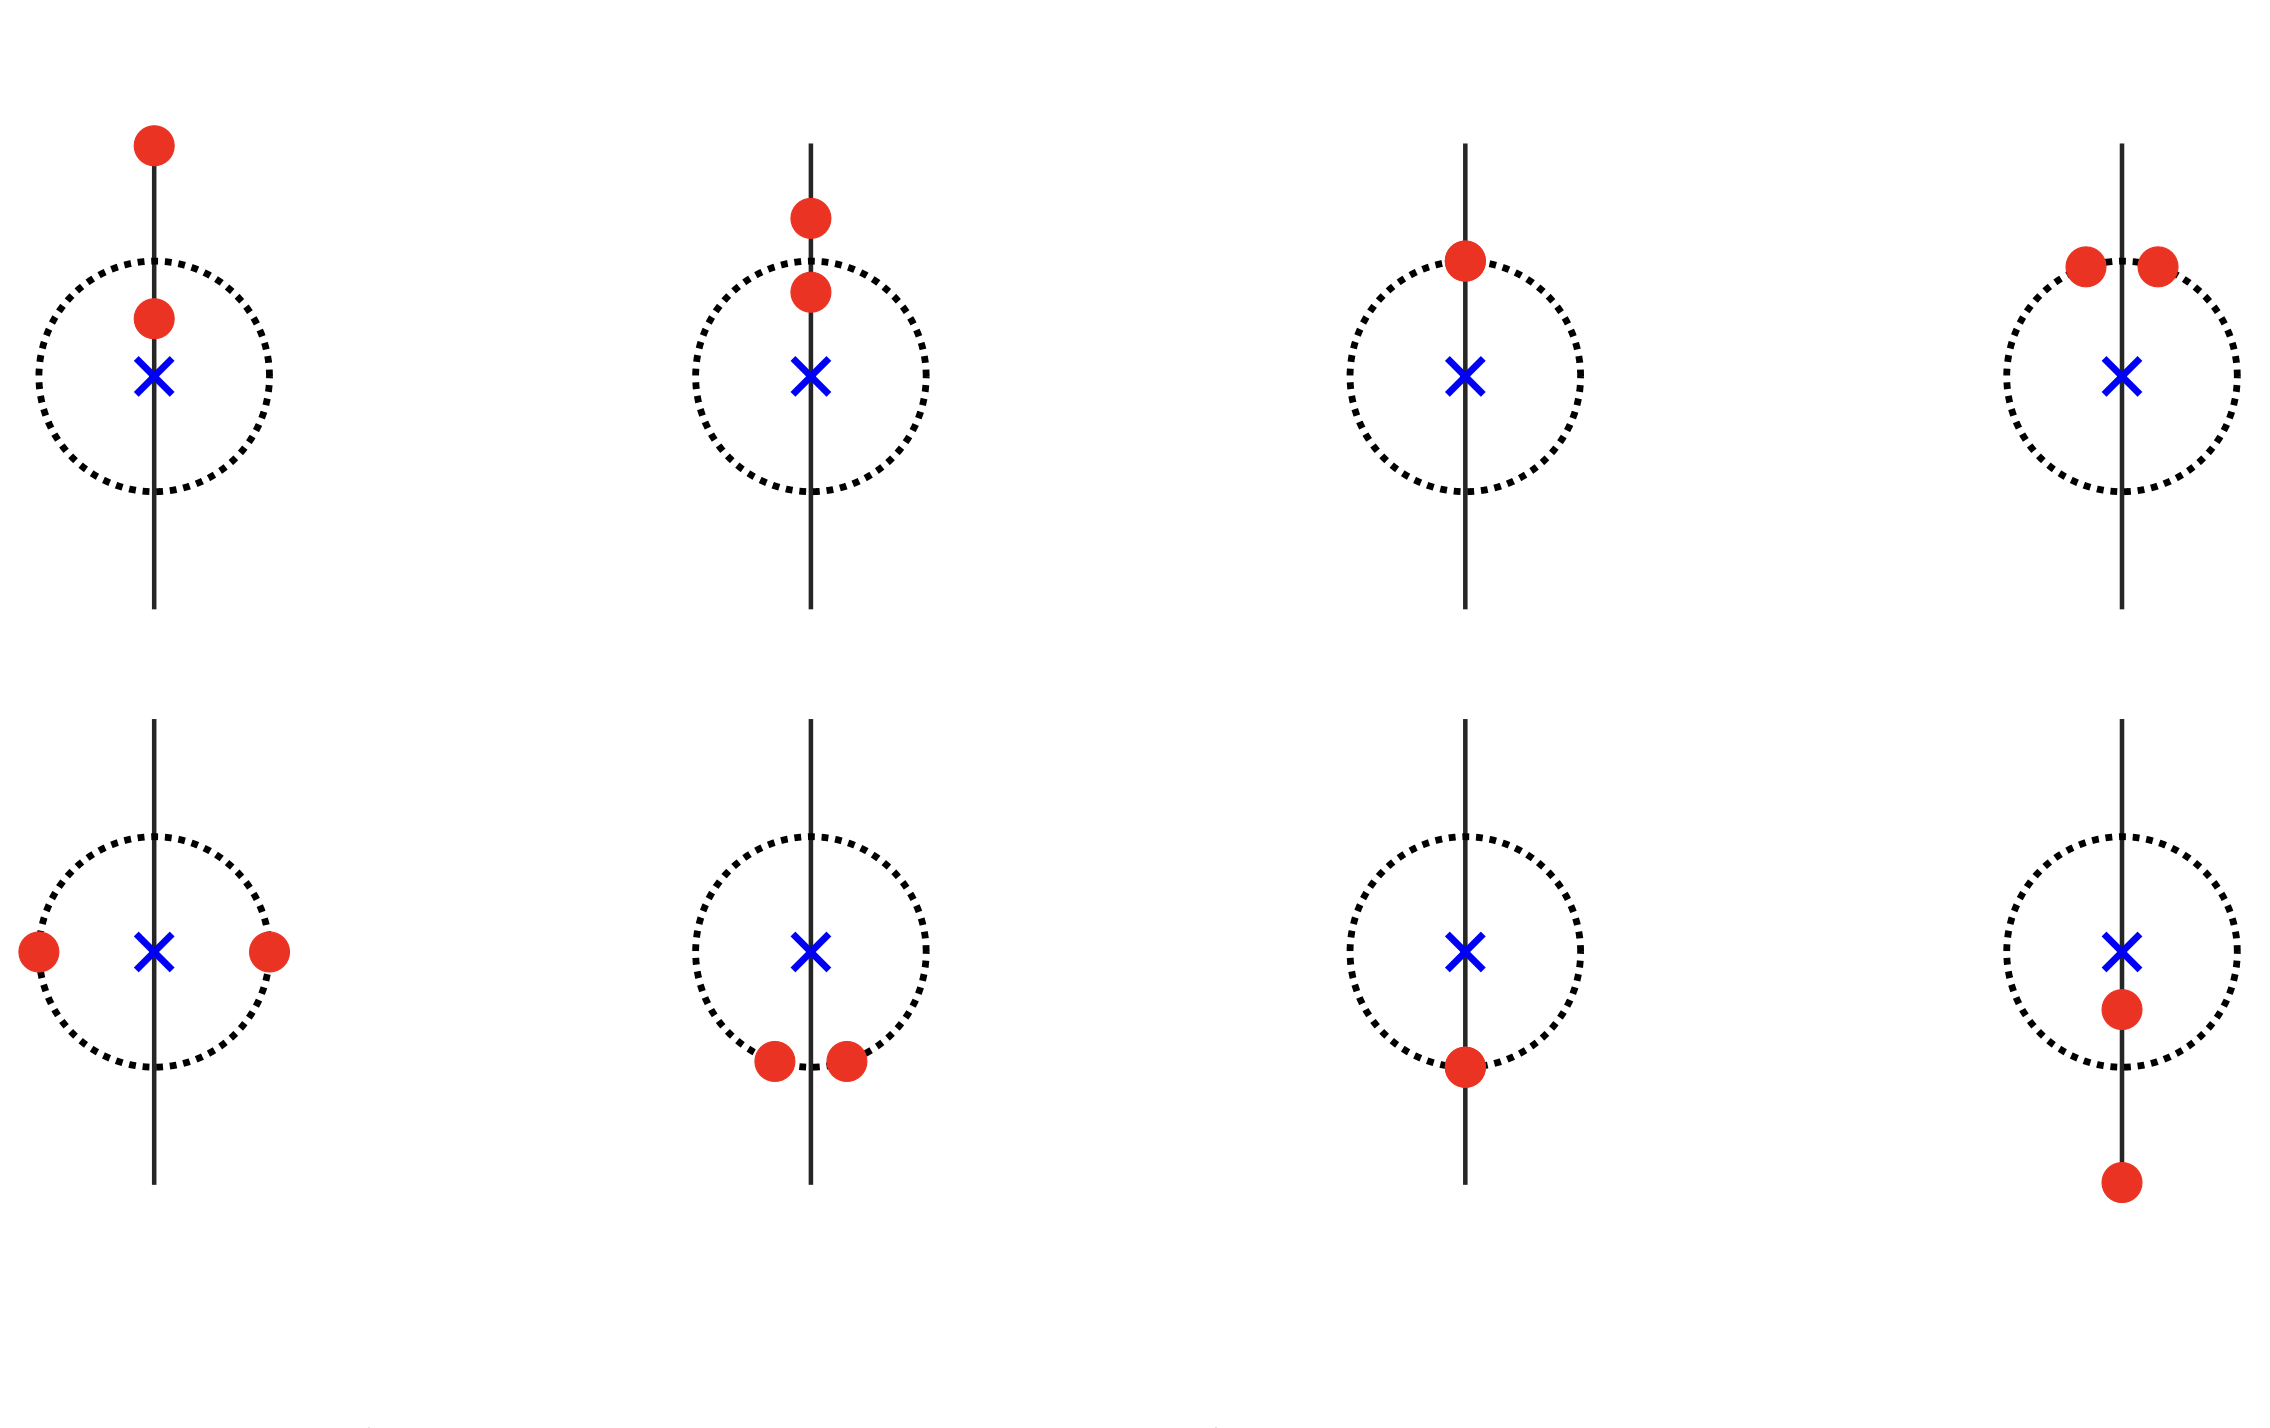
\includegraphics[width=9cm]{images/KreinBubbleCartoonSS2.png} & 
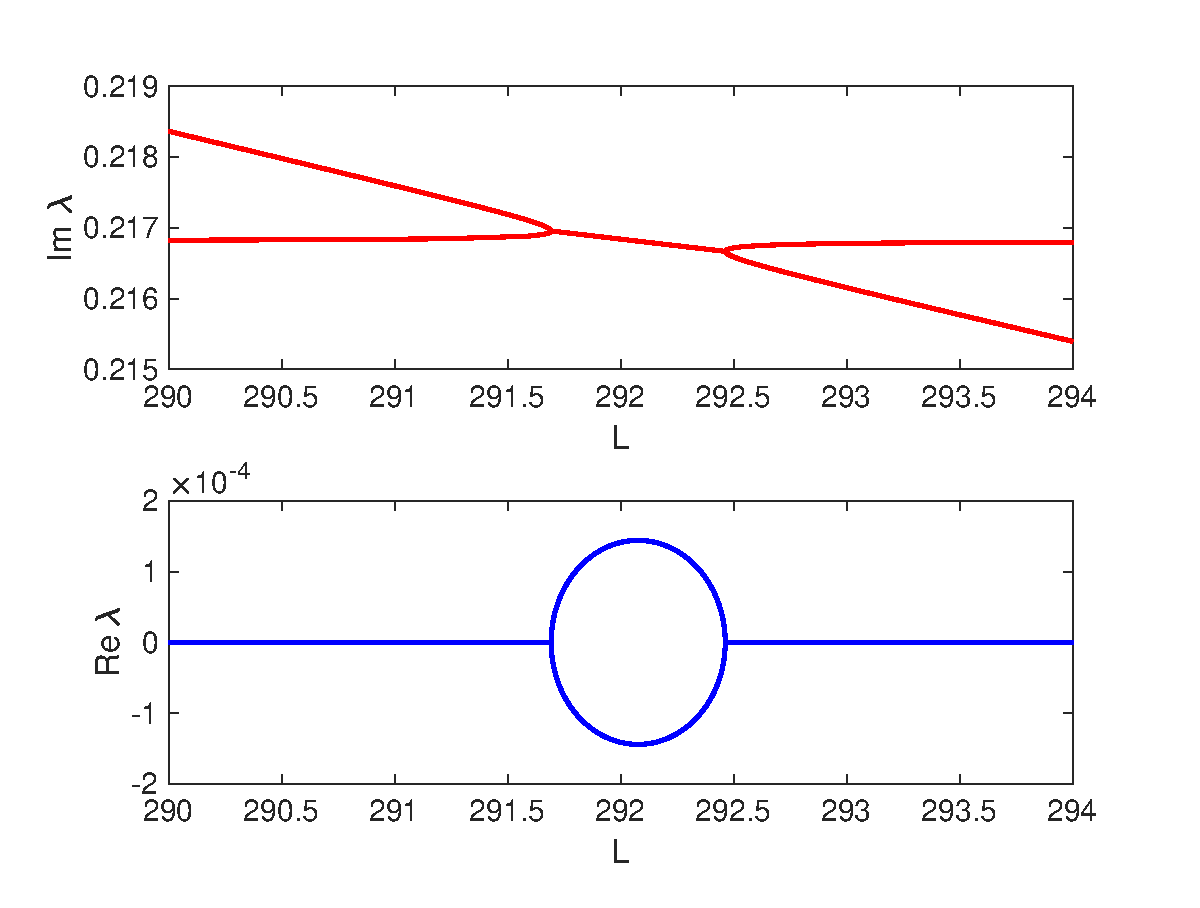
\includegraphics[width=8cm]{images/kreinbubble1.eps}
\end{tabular}
\end{center}
\caption{Krein instability bubble cartoon (left) and numerical simulation for KdV5 (right).}
\label{fig:kreinbubble1}
\end{figure}

\subsection*{Fourth order nonlinear Schr\"odinger equation}

The following fourth-order nonlinear Schr{\"o}dinger equation
\begin{align*}
    i u_t + \frac{\beta_4}{24}u_{xxxx} - \frac{\beta_2}{2}u_{xx} + \gamma |u|^2 u &= 0 
\end{align*}
is a variant of the nonlinear Schr{\"o}dinger equation which was introduced to account for the role of small fourth-order dispersion terms in the propagation of intense laser beams in a bulk medium with Kerr nonlinearity \cite{Karpman2000,Tam2020}. Motivated by recent experiments \cite{Tam2019}, there is particular interest in the case where $\beta_2 = 0$, in which case the system exhibits pure quartic dispersion; the resulting solitary wave solutions are known as pure quartic solitons (PQS). I prove that while multi-pulse solitary wave solutions exist, they are all unstable due to the presence of at least one interaction eigenvalue with positive real part \cite[Theorems 1 and 2]{Parker2020NLS4}. To confirm these results numerically, I obtain PQS solutions by using numerical parameter continuation with a conjugate gradient solver, and perform time evolution simulations on perturbations of solitary wave solutions using a split-step Fourier method. The evolution of these perturbations can be explained by the interaction eigenvalues and their corresponding eigenfunctions. Future work includes extending the model to incorporate a term characterizing Raman scattering, which leads to symmetry distortion and reduced pulse amplitude, as well as terms corresponding to gain and loss of energy. Since PQS are an active area of experimental research, parameters in the model could also be fit to experimental results. Another avenue of research would be to study a fourth order version of the generalized Lugiato-Lefever equation (GLLE), which is similar to NLS but contains a convolution term to model nonlocal effects.

\subsection*{Other systems and future directions}

Other systems of interest include the discrete sine-Gordon equation, nonlocal lattice equations, and equations on higher dimensional lattices. The discrete sine-Gordon equation
\begin{align*}
    \frac{d^2}{dt^2}u_n &= d (\Delta_2 u)_n - \sin(u_n) && n \in \mathbb{Z}
\end{align*}
was introduced to describe the dynamics of crystal lattices, and has since been used in numerous applications, including a mechanical model for a chain of pendulums coupled with elastic springs, arrays of Josephson junctions, and DNA dynamics \cite{braun2004}. A particular class of coherent structures in this system are kinks, which are exponentially localized stationary solutions that connect adjacent minima of the potential $V(u) = \cos u$. Using similar techniques as with multi-pulses, I prove the existence of stationary multi-kink solutions as well as analyze their spectral stability \cite{parkerSG}. Another important class of coherent structures is breathers, which are localized, oscillatory patterns. Future work involves using Lin's method to construct multi-site breathers by splicing together multiple, sequential copies of the primary breather, and then analyzing their spectral stability. As a first step, both the primary breather solution and multi-site breathers can be computed using either numerical parameter continuation or a shooting method. The spectrum can then be computed using a numerical eigenvalue solver.

Finally, one nonlocal version of DNLS is
\begin{align*}
    i \frac{d}{dt} u_n = \frac{1}{h^{2s}} \sum_{m \neq n} \frac{u_m - u_n}{|m - n|^{1+2s}} + |u_n|^2 u_n && n \in \mathbb{Z},
\end{align*}
where $s > 0$ is a fixed parameter specifying the decay of the nonlocal interactions \cite{Kirkpatrick2013}. In the continuum limit $h\rightarrow 0$, this equation converges to an NLS equation with fractional Laplacian \cite{Kirkpatrick2013}. Applications include a model for charge transport in DNA polymers. Future directions include studying solitary wave and multi-pulse solutions in this system, as well as whether the nonlocal interaction term permits other solutions which are not found in DNLS. A final, related area of interest is coherent structures in DNLS on the square integer lattice $\mathbb{Z}^2$, which could include nonlocal interactions in one or both directions. 

\section*{Coherent structures in optical lattices}

There has been much recent interest in the field of topological photonics, as experimental physicists and engineers have developed new techniques for controlling light propagation in photonic crystals and optical fibers. One specific application is light transmission through multi-core optical fibers. In particular, optical transmission properties can be tuned by introducing a twist to the fiber bundle \cite{Longhi2016,CastroCastro2016,Parto2017} (\cref{fig:twist}, top).
\begin{figure}
\begin{center}
\begin{tabular}{cc}
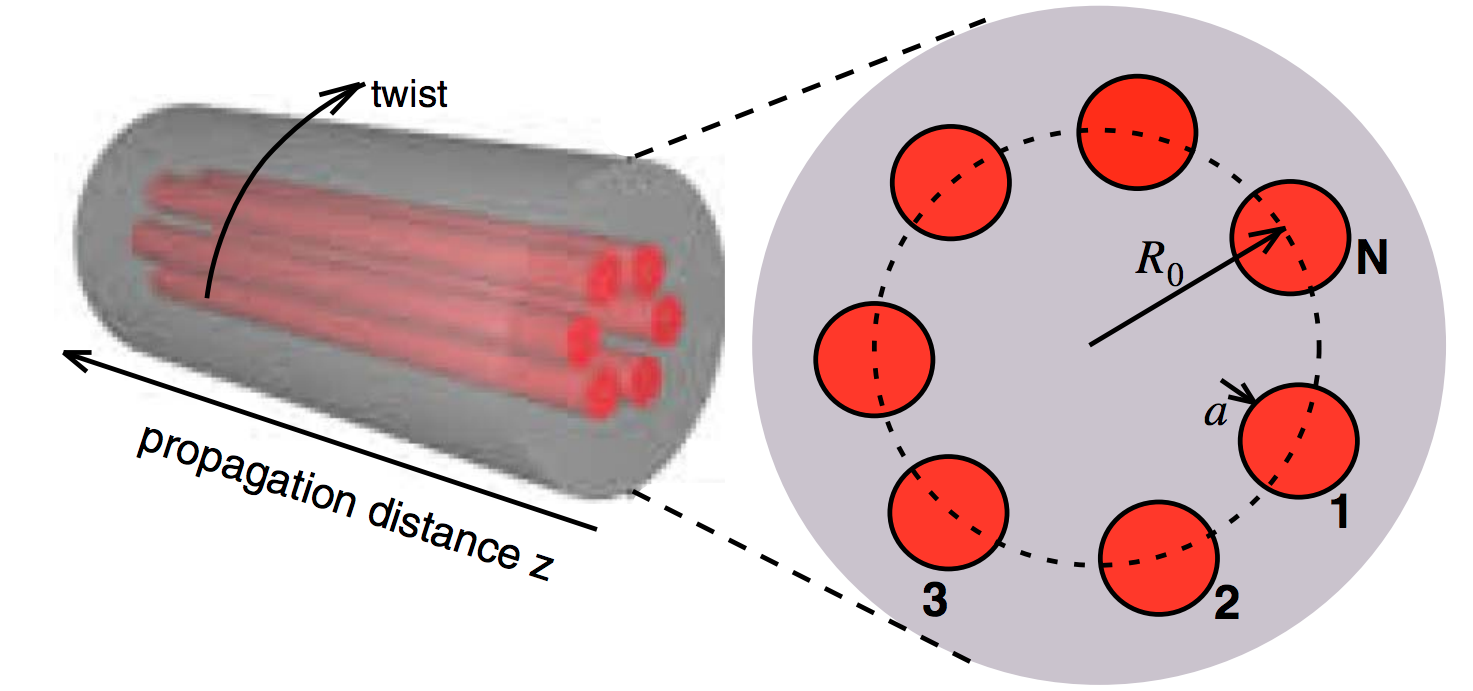
\includegraphics[width=7cm]{images/twist2.png} &
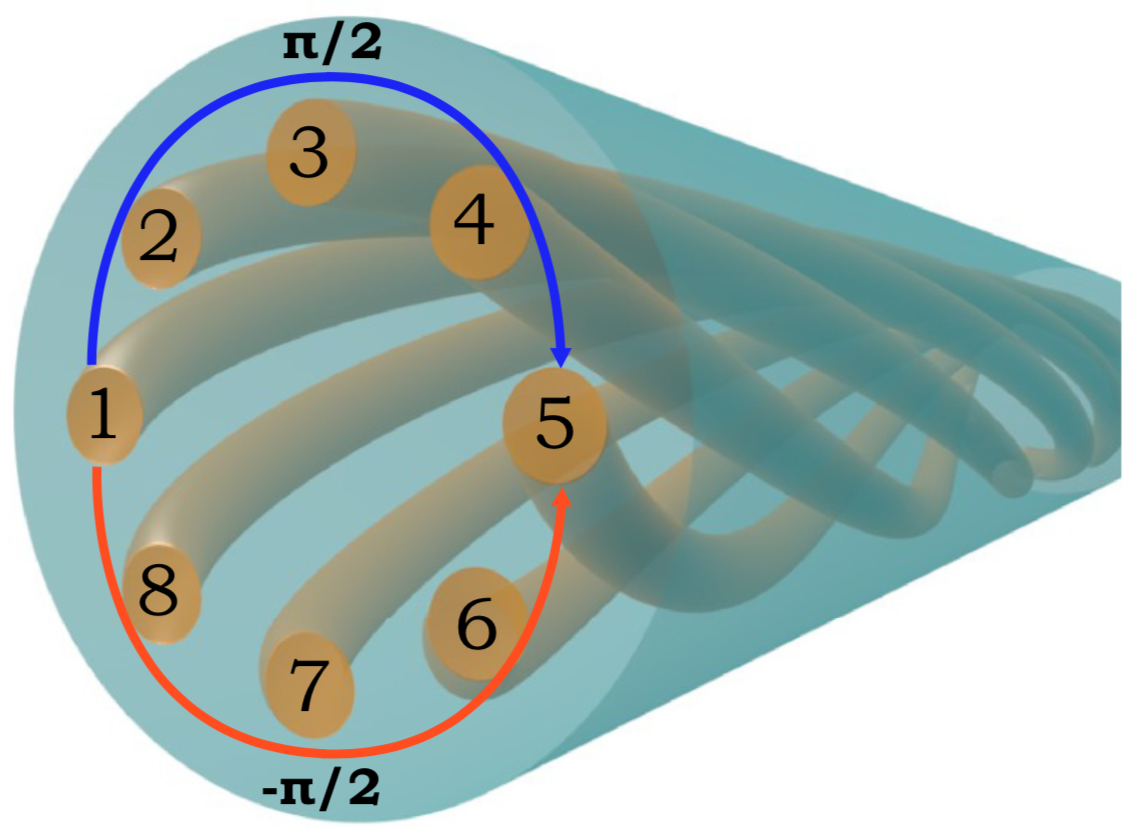
\includegraphics[width=4.25cm]{images/twistmulticore.png} \\
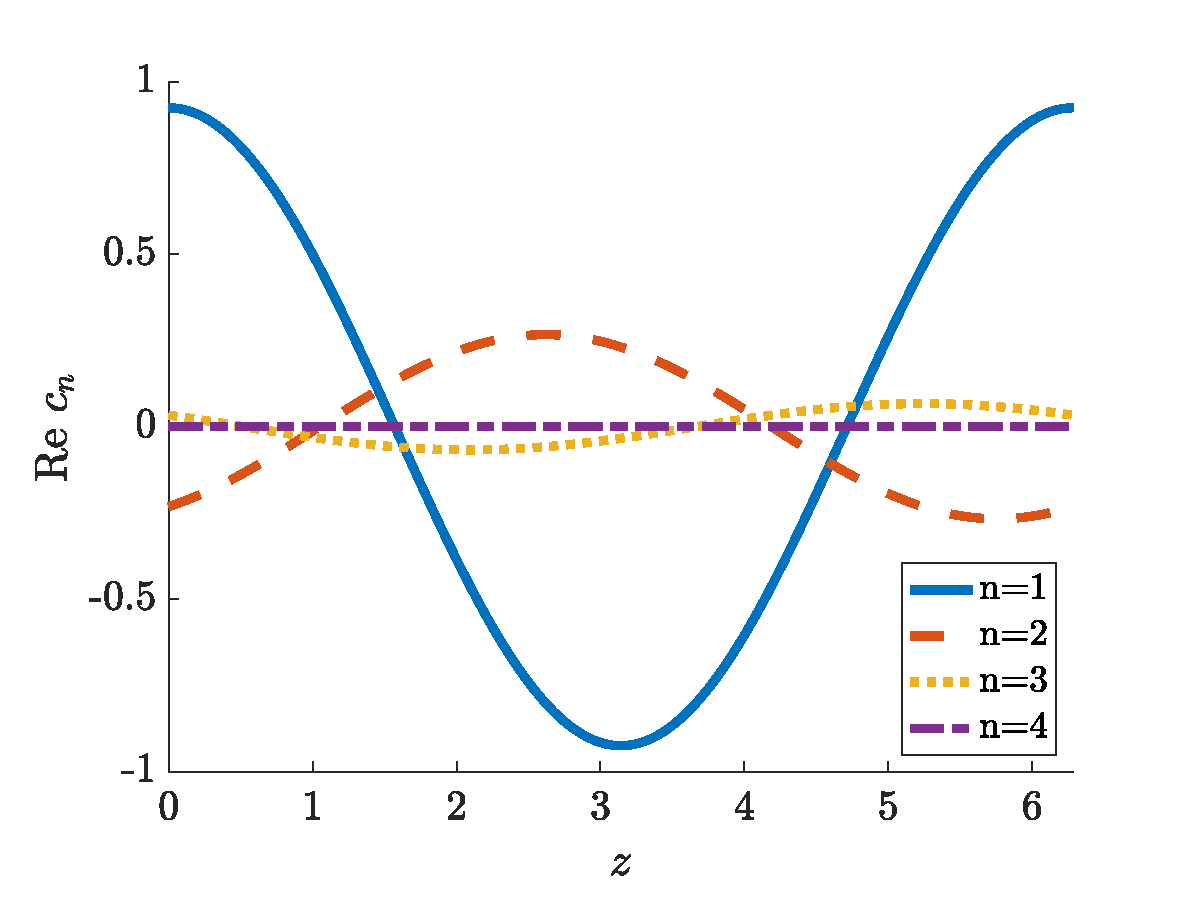
\includegraphics[width=7cm]{images/evenholestandingwave.eps} &
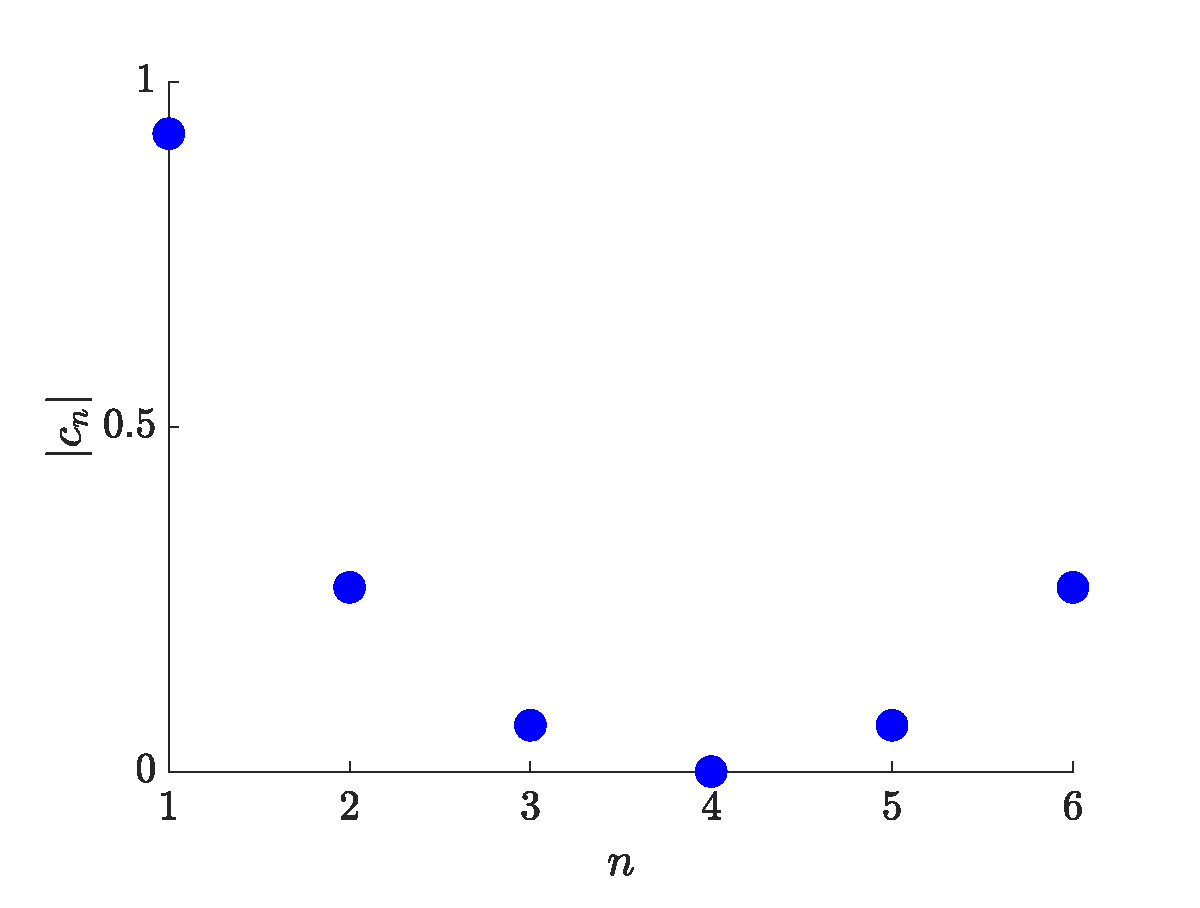
\includegraphics[width=7cm]{images/evenholeamps.eps}
\end{tabular}
\end{center}
\caption{Circular multi-core fiber \cite{Longhi2016} (top left) and twisted multi-core fiber with eight waveguides \cite{Parto2017} (top right). Bottom panel shows standing wave solution for twisted multi-core fiber with $N = 6$ and $\phi = \pi/6$, with evolution of real part of solution for first four sites on bottom left and magnitude of solution at the sites on bottom right. Site 1 has maximum intensity, and opposite site 4 has zero intensity.}
\label{fig:twist}
\end{figure}
The propagation of light through a twisted optical fiber comprising $N$ waveguides arranged in a circle is described by the coupled mode equations
\begin{align*}
i \frac{d}{dz} c_n &= k \left(e^{-i\phi}c_{n+1} + e^{i\phi}c_{n-1}\right) + |c_n|^2 c_n &&  n = 1, \dots, N,
\end{align*}
where $z$ is the axis of propagation, $k$ is the strength of the nearest-neighbor coupling, and $\phi$ is a parameter representing the twist of the fiber.  When the twist parameter $\phi$ and the number of fibers $N$ are related by $\phi = \pi/N$, I prove that there is a stable standing wave solution of the form $c_n(z) = a_n e^{i \omega z}$ which has a ``dark node'' with no optical activity (node 4 in \cref{fig:twist}, bottom) opposite a ``bright node'' of maximum intensity (node 1 in \cref{fig:twist}, bottom) \cite{ParkerTwist}. To do this, I first used numerical parameter continuation to compute standing wave solutions. This showed me what types of solutions to expect and the symmetry relationships between the fibers in the bundle. Using these symmetries, I derived an algebraic relationship between the fiber intensities, which I then solved using the implicit function theorem. I recently extended this result by using asymptotic analysis to demonstrate that the same suppression effect occurs if the model involves a temporal dispersion term \cite{ParkerSpatiotemporalTwist}.

Newer work involves studying coherent structures in more complicated arrays of optical fibers, and correlating the results from the mathematical models with experimental data. One example is a waveguide consisting of a square lattice of fibers, in which there are periodic variations along the waveguide axis causing the nearest-neighbor coupling to vary periodically in $z$ \cite{Mukherjee2020}. In particular, for any $z$, a waveguide is coupled to only one of its four neighbors (\cref{fig:Rechtsman}, left). This configuration gives rise to localized periodic breather solutions, in which the bulk of the optical intensity is confined to a single square in the lattice but ``jumps'' around that square counterclockwise (\cref{fig:Rechtsman}, center and right). In some recent work, I perform a systematic numerical analysis of the existence and stability of localized solutions in this system and conclude that some of these structues are stable \cite{parker2021Floquet}.
Other arrangements of fibers which are of interest to experimentalists include concentric rings and honeycomb lattices \cite{Lumer2013}. This research would introduce students to many different computational techniques, including numerical parameter continuation, shooting methods, and energy minimization methods to generate solutions; eigenvalue solvers to compute the spectrum of the linearization of the system about that solution; and numerical ODE and PDE solvers to study how perturbations of the solution evolve in time. 
\begin{figure}
    \centering
    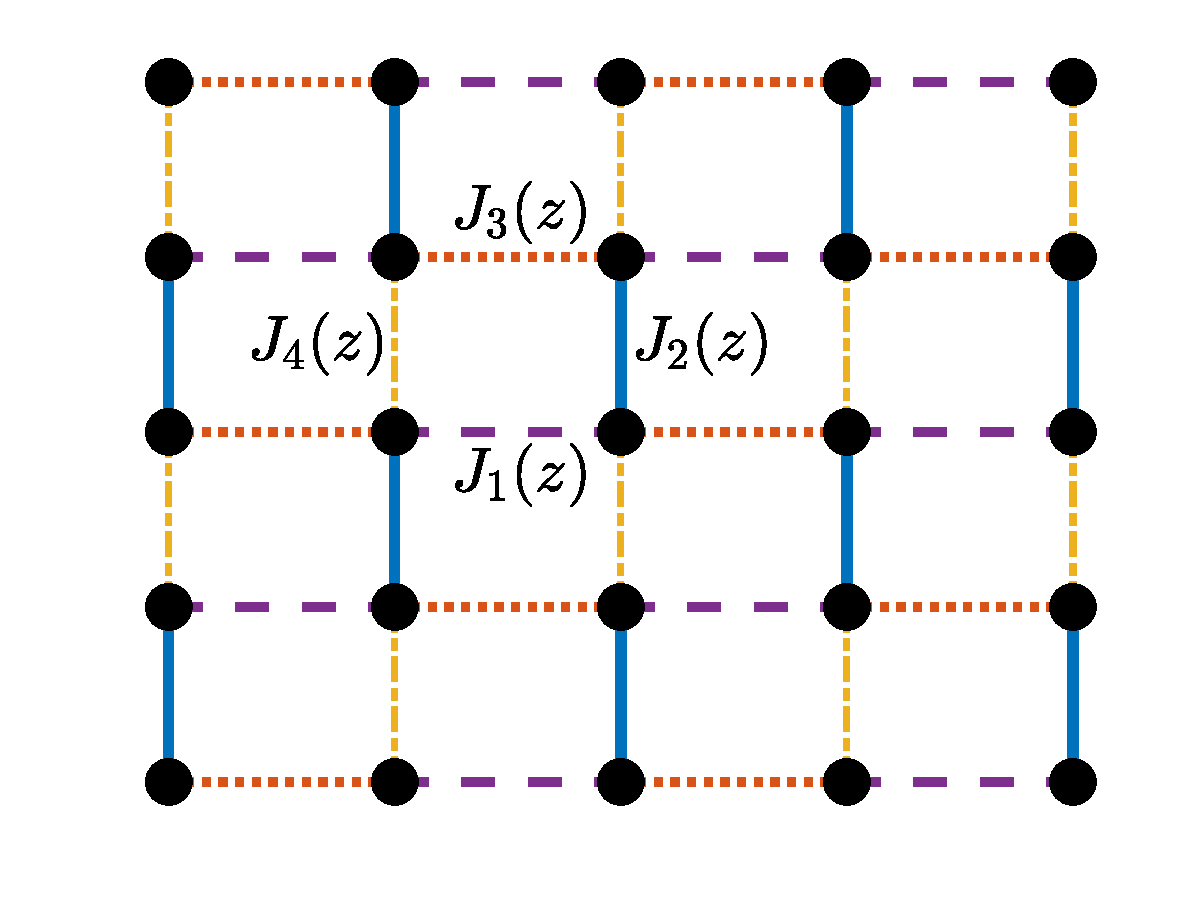
\includegraphics[width=6cm]{images/lattice.eps}\hspace{-0.6cm}
    % 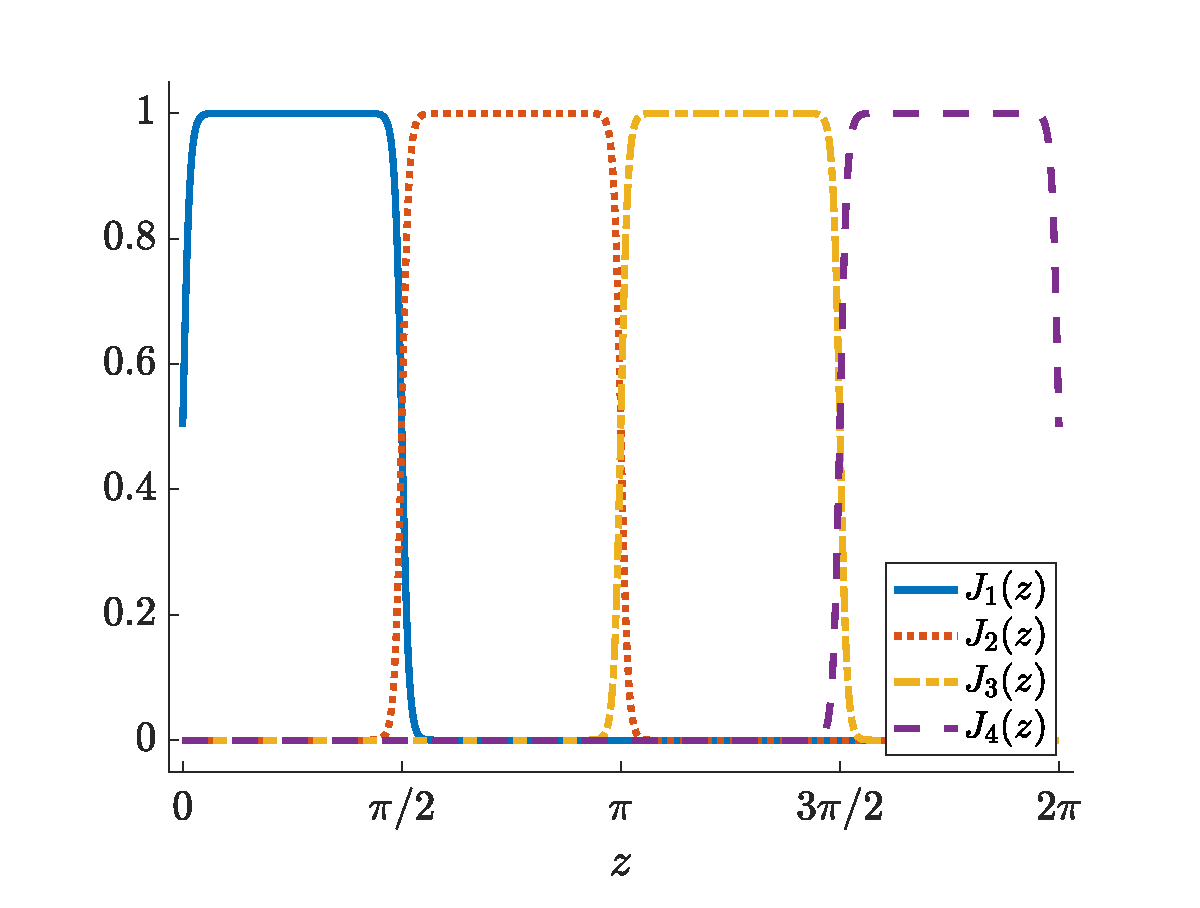
\includegraphics[width=7.8cm]{images/Jplot.eps}
    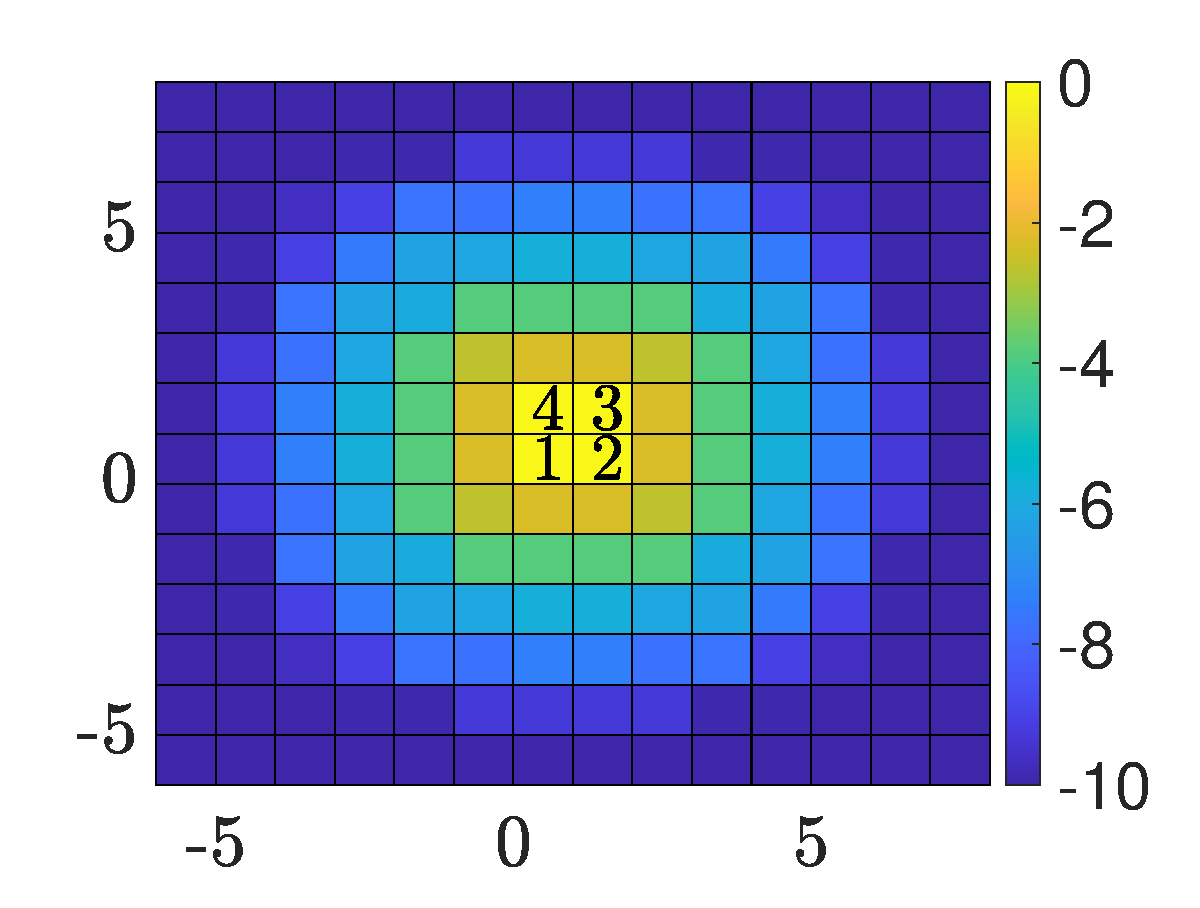
\includegraphics[width=6cm]{images/fundc1map.eps}\hspace{-0.4cm}
    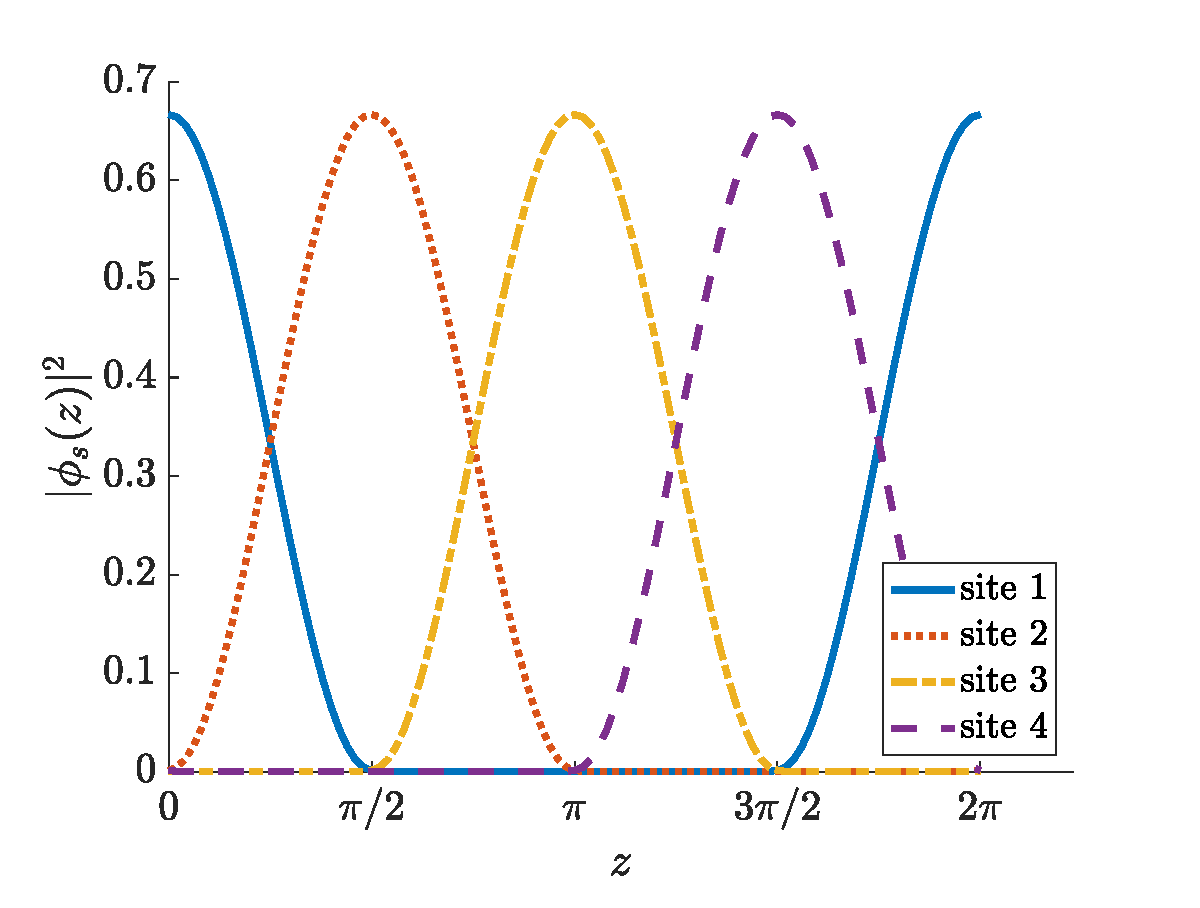
\includegraphics[width=6cm]{images/fundc1sol.eps}
    \caption{Cartoon of square lattice with $z$-dependent coupling (left). At any value of $z$, only one of the four coupling functions $J_k(z)$ is nonzero. Log intensity of fundamental breather solution over one period, showing localization to a single unit square in lattice (center). Square intensity of fundamental breather solution on the unit square over one period (right).}
    \label{fig:Rechtsman}
\end{figure} 

\section*{Bifurcations in neural models}

Finally, some current work involves studying bifurcations in a model of a neural network
\begin{equation*}
    \dot{\xvec} = -\xvec  + \frac{1}{\sqrt{N}} H\tanh (g \xvec),
\end{equation*}
where $\xvec = (x_1, \dots, x_N)$ represents the firing rate of each neuron in the network \cite{ParkerNeuro,Barreiro2017}. The network topology and neuronal connection weights are specified by the connectivity matrix $H$, and the individual neurons are connected using a sigmoidal hyperbolic tangent activation function. Adjusting the parameter $g$, which represents the global connection strength, leads to bifurcations, in which the stability and number of equilibrium points in the system change; periodic solutions may also emerge at these bifurcation points. The specific bifurcation structure depends on symmetries in the matrix $H$. 

For one example, suppose the neurons are grouped into two clusters, one containing excitatory cells and the other containing inhibitory cells. When $g = 0$, the origin is a stable equilibrium point of the system. As $g$ is increased, the origin loses stability in a symmetric pitchfork bifurcation (filled circle in \cref{fig:neuroBD}). Multiple branches of equilibrium points emerge from this bifurcation point due to the symmetries of $H$. As $g$ is further increased, there is a Hopf bifurcation (filled squares in \cref{fig:neuroBD}) on each branch of equilibria, after which point periodic orbit solutions are found. At a critical value of $g$, these limit cycles coalesce (dark band in \cref{fig:neuroBD}), after which point the system only has a single stable limit cycle. To locate equilibria and bifurcation points, and to compute periodic solutions, I use numerical parameter continuation with AUTO. I then use these numerical results as a starting point for theoretical work. For example, the parameter continuation results suggested a perturbation method that I used to prove the Hopf bifurcations in \cref{fig:neuroBD} exist, and to determine their location to leading order. Future work with students could include exploring symmetries and bifurcations in the model resulting from other groupings of neurons, as well as studying the effects of noise on the model. This research would introduce students to numerical continuation and perturbation methods, which are two essential tools in computational and applied mathematics.

\begin{figure}
    \centering
    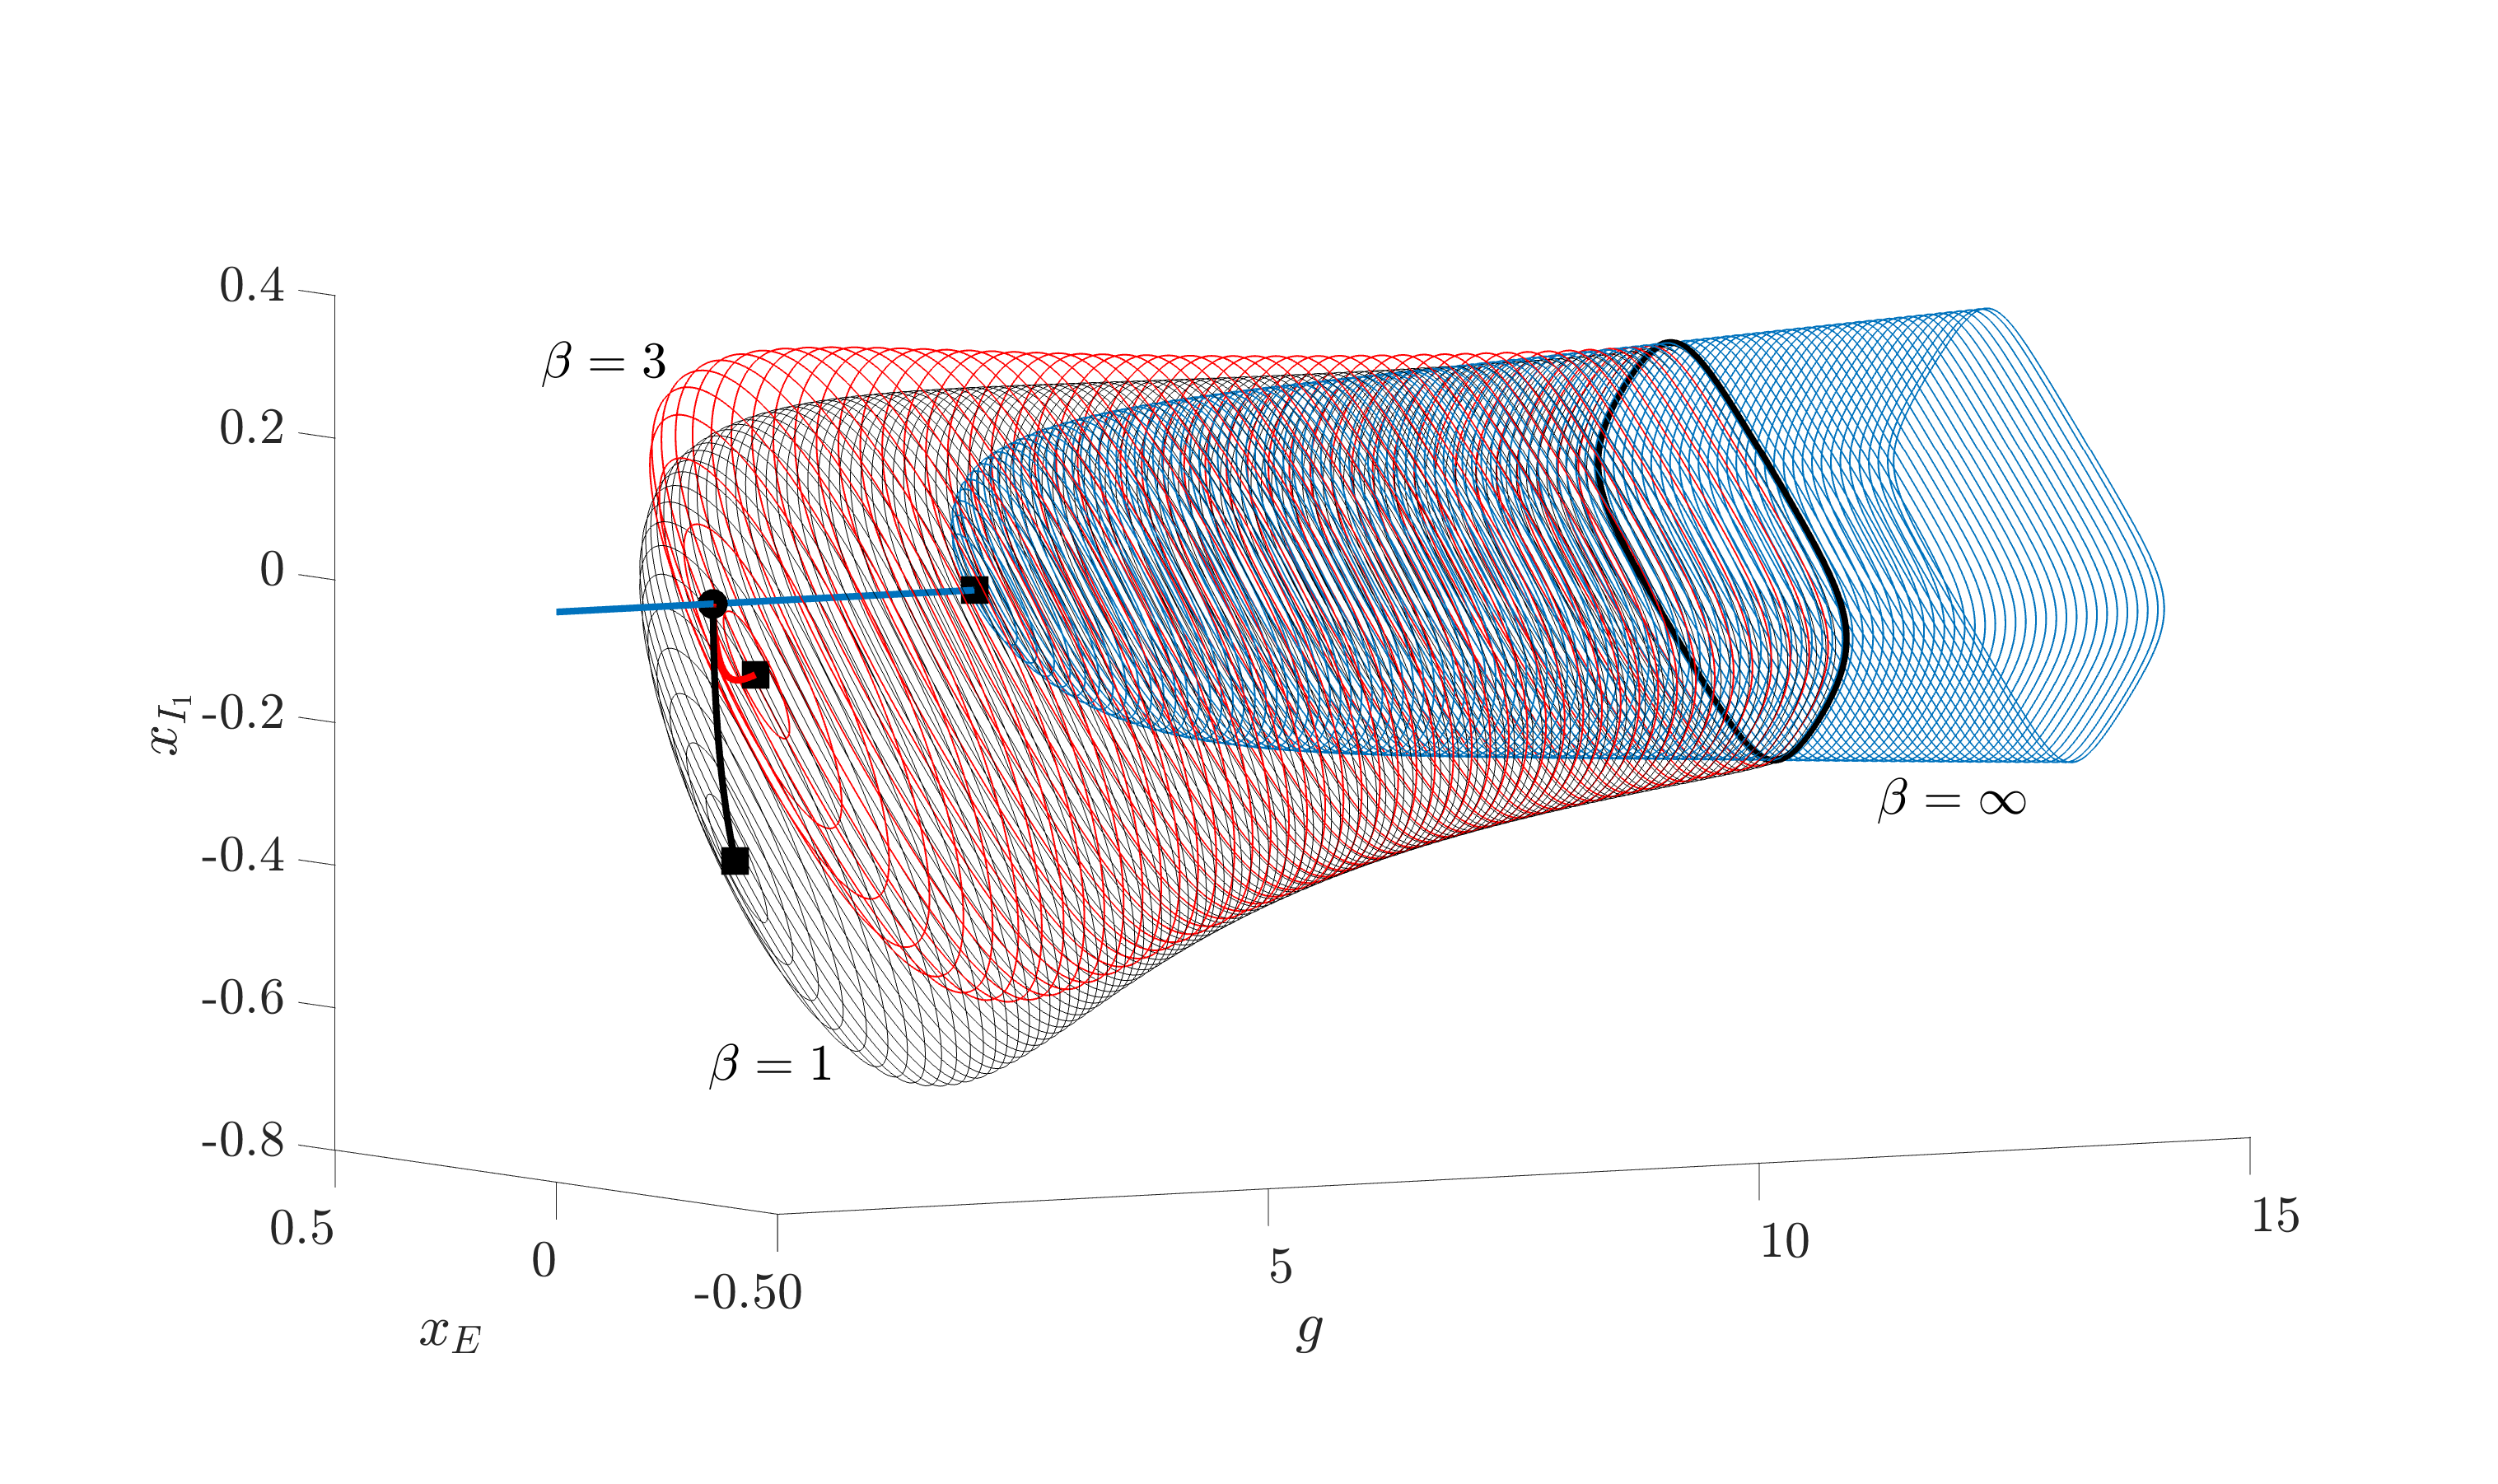
\includegraphics[width=14cm]{images/pitchbif.eps}
    \caption{Bifurcation structure of neural network model as the connection strength parameter $g$ is increased, showing fixed points (solid lines) and periodic orbits (rings). Symmetric pitchfork bifurcation indicated with filled circle. Hopf bifurcations indicated with filled squares.}
    \label{fig:neuroBD}
\end{figure}

% \subsection*{Coupled oscillators}

% In the summer of 2021, I supervised an REU in which undergraduate students learned about different coupled oscillator models and then designed their own research projects to explore these models computationally. One example is the Kuramoto model
% \begin{align*}
% \frac{d \theta_j}{dt} = \omega_j + \frac{K}{N}\sum_{k=1}^N \sin(\theta_k - \theta_j) && j = 1, \dots N,
% \end{align*}
% which was developed to study synchronization in systems of chemical and biological oscillators; it has numerous  applications, including circadian rhythms, chirping crickets, and flashing fireflies. The model describes a set of $N$ oscillators with phases $\theta_j$ and natural frequencies $\omega_j$. Every oscillator is connected to every other oscillator using a nonlinear sinusoidal function, and the parameter $K$ controls the strength of this coupling. For a critical value of $K$, which depends on the initial distribution of natural frequencies $\omega_j$, the oscillators will start to synchronize, despite their different natural frequencies \cite{strogatz2000}. As the model evolves in time, the degree of synchrony can be measured by computing the complex order parameter
% \[
% r e^{i \psi} = \frac{1}{N}\sum_{j=1}^N \mathrm{e}^{i \theta_j},
% \]
% which characterizes the ``collective rhythm'' of the oscillators \cite{strogatz2000}. The modulus $r$ quantifies the phase coherence, with $r = 0$ representing no synchrony, and $r = 1$ representing complete synchrony. My students found that as the coupling parameter $K$ is rapidly varied, the system gains synchrony faster when $K$ is increased than it loses synchrony when $K$ is decreased. This hysteresis effect is shown in \cref{fig:KuramotoK}. They will present their results on a poster at the regional SIAM TX-LA conference. Future work with students includes examining models in which the connections between oscillators are specified by an adjacency matrix, and exploring a second-order variant of the Kuramoto model \cite{Grzybowski2016} which has applications to electrical power grids. 

% \begin{figure}[H]
%     \centering
%     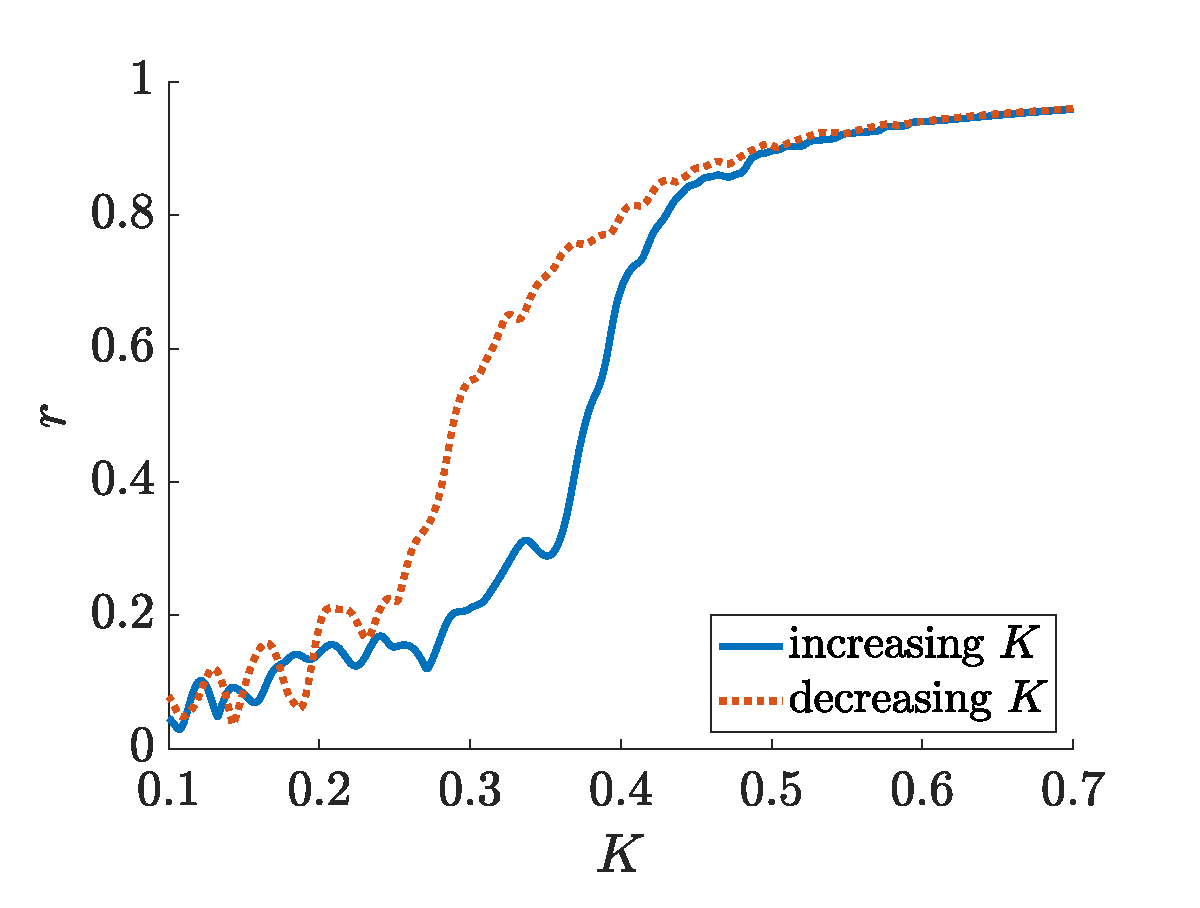
\includegraphics[width=8cm]{images/KuramotoK.eps}  
%     \caption{Order parameter $r$ vs coupling parameter $K$, as $K$ is increased (solid blue line) then decreased (dotted orange line). Figure courtesy Jerry Luckenbaugh and Jamie Moseley.}
%     \label{fig:KuramotoK}
% \end{figure}

\pagebreak
\bibliographystyle{siam}
\footnotesize{ \bibliography{researchstatement.bib} }

\end{document}
